%==============================================================================
%  SBS Data Factory — Plateforme Drive-to-Store DSP
%  Rapport de Projet de Fin d'Année (PFA) / Stage
%  Auteure : Aya ACHIBAN — ENSAM Casablanca — Année universitaire 2025/2026
%
%  Compilation recommandée (voir README.md) :
%     xelatex rapport-final-stage.tex   (deux passes pour la table des matières)
%  Compatible également avec pdfLaTeX (préambule conditionnel via iftex).
%  Aucun paquet nécessitant --shell-escape n'est utilisé.
%==============================================================================
\documentclass[11pt,a4paper,oneside]{report}

%------------------------------------------------------------------------------
% Moteur : préambule conditionnel (compatible pdfLaTeX et XeLaTeX/LuaLaTeX)
%------------------------------------------------------------------------------
\usepackage{iftex}
\ifPDFTeX
  \usepackage[utf8]{inputenc}
  \usepackage[T1]{fontenc}
  \usepackage{lmodern}
\else
  \usepackage{fontspec}
\fi

%------------------------------------------------------------------------------
% Langue
%------------------------------------------------------------------------------
\usepackage[french]{babel}
\usepackage{csquotes}

% Libellés français normalisés : « Tableau » plutôt que « Table » pour les
% légendes, et titres homogènes pour les listes de figures et de tableaux.
\addto\captionsfrench{%
  \renewcommand{\tablename}{Tableau}%
  \renewcommand{\listfigurename}{Liste des figures}%
  \renewcommand{\listtablename}{Liste des tableaux}%
}

% Les noms propres techniques ne doivent jamais être coupés en fin de ligne.
\hyphenation{ENSAM PostgreSQL OpenStreetMap FastAPI JavaScript Swagger
  OpenAPI GitHub Recharts Leaflet Pydantic SQLAlchemy Tailwind Uvicorn}

%------------------------------------------------------------------------------
% Mise en page
%------------------------------------------------------------------------------
\usepackage[a4paper,top=2.6cm,bottom=2.6cm,left=2.6cm,right=2.4cm,headheight=15pt]{geometry}
\usepackage{setspace}
\onehalfspacing

% Micro-typographie : justification plus régulière, moins de coupures et
% d'espaces disgracieux (compatible pdfLaTeX et XeLaTeX).
\usepackage{microtype}

% Tolérance de justification accrue (préférable à \sloppy, qui produit des
% espaces inter-mots trop lâches).
\tolerance=2000
\emergencystretch=1.5em

%------------------------------------------------------------------------------
% Graphismes et couleurs
%------------------------------------------------------------------------------
\usepackage{graphicx}
\usepackage{xcolor}
\usepackage{float}
\usepackage{caption}
\usepackage{subcaption}
\usepackage{tikz}
\usetikzlibrary{shapes.geometric,arrows.meta,positioning,fit,backgrounds}

\graphicspath{{../rapport-final-assets/screenshots/}{../rapport-final-assets/logos/}}

% Palette SBS : marine sombre + accents violet / or (sobre)
\definecolor{sbsnavy}{HTML}{0F172A}
\definecolor{sbspurple}{HTML}{5A2FBE}
\definecolor{sbspurplesoft}{HTML}{7E51E8}
\definecolor{sbsgold}{HTML}{C9A227}
\definecolor{sbslight}{HTML}{F4F1FE}
\definecolor{sbsgray}{HTML}{475569}
\definecolor{sbsline}{HTML}{CBD5E1}

%------------------------------------------------------------------------------
% Tableaux
%------------------------------------------------------------------------------
\usepackage{booktabs}
\usepackage{longtable}
\usepackage{array}
\usepackage{tabularx}
\usepackage{enumitem}
\setlist{itemsep=2pt,topsep=3pt}

% Colonne X justifiée à gauche pour tabularx
\newcolumntype{L}{>{\raggedright\arraybackslash}X}

%------------------------------------------------------------------------------
% Code source (listings — pas de shell-escape)
%------------------------------------------------------------------------------
\usepackage{listings}
\lstdefinestyle{sbscode}{
  basicstyle=\ttfamily\footnotesize,
  backgroundcolor=\color{sbslight},
  frame=single,
  rulecolor=\color{sbsline},
  keywordstyle=\color{sbspurple}\bfseries,
  commentstyle=\color{sbsgray}\itshape,
  stringstyle=\color{sbsgold!80!black},
  numbers=none,
  breaklines=true,
  showstringspaces=false,
  columns=fullflexible,
  keepspaces=true,
  xleftmargin=8pt,
  xrightmargin=4pt,
  aboveskip=8pt,
  belowskip=8pt,
}
\lstset{style=sbscode}

\ifPDFTeX
  % pdfLaTeX : sans cette table, les caractères accentués des listings sont
  % silencieusement perdus (« Créer » devenait « Crer » dans le PDF).
  \lstset{literate=%
    {é}{{\'e}}1 {è}{{\`e}}1 {ê}{{\^e}}1 {ë}{{\"e}}1
    {à}{{\`a}}1 {â}{{\^a}}1 {î}{{\^i}}1 {ï}{{\"i}}1
    {ô}{{\^o}}1 {ö}{{\"o}}1 {ù}{{\`u}}1 {û}{{\^u}}1 {ü}{{\"u}}1
    {ç}{{\c{c}}}1 {É}{{\'E}}1 {È}{{\`E}}1 {À}{{\`A}}1 {Ç}{{\c{C}}}1
  }
\fi

%------------------------------------------------------------------------------
% Titres de sections/chapitres
%------------------------------------------------------------------------------
\usepackage{titlesec}
\titleformat{\chapter}[display]
  {\normalfont\bfseries}
  {\filright\large\color{sbspurple}\MakeUppercase{\chaptertitlename}\ \thechapter}
  {0.6ex}
  {\color{sbsnavy}\huge\filright}
  [\vspace{0.6ex}{\color{sbsgold}\titlerule[1.2pt]}]
\titlespacing*{\chapter}{0pt}{6pt}{22pt}

\titleformat{\section}
  {\normalfont\large\bfseries\color{sbsnavy}}{\thesection}{0.6em}{}
\titleformat{\subsection}
  {\normalfont\normalsize\bfseries\color{sbspurple}}{\thesubsection}{0.6em}{}

%------------------------------------------------------------------------------
% En-têtes / pieds de page
%------------------------------------------------------------------------------
\usepackage{fancyhdr}
\pagestyle{fancy}
\fancyhf{}
\fancyhead[L]{\small\color{sbsgray}\nouppercase{\leftmark}}
\fancyhead[R]{\small\color{sbsgray}SBS Drive-to-Store DSP}
\fancyfoot[C]{\small\color{sbsnavy}\thepage}
\renewcommand{\headrulewidth}{0.4pt}
\renewcommand{\footrulewidth}{0pt}
\renewcommand{\headrule}{\hbox to\headwidth{\color{sbsline}\leaders\hrule height \headrulewidth\hfill}}

\fancypagestyle{plain}{%
  \fancyhf{}
  \fancyfoot[C]{\small\color{sbsnavy}\thepage}
  \renewcommand{\headrulewidth}{0pt}
}

%------------------------------------------------------------------------------
% Légendes de figures / tableaux
%------------------------------------------------------------------------------
\captionsetup{font=small,labelfont={bf,color=sbspurple},labelsep=colon,
  justification=centering}

%------------------------------------------------------------------------------
% Liens hypertextes (chargé tardivement)
%------------------------------------------------------------------------------
\PassOptionsToPackage{hyphens}{url}% URLs longues : autoriser la coupure
\usepackage{hyperref}
\hypersetup{
  unicode=true,
  colorlinks=true,
  linkcolor=sbsnavy,
  citecolor=sbspurple,
  urlcolor=sbspurple,
  pdftitle={Rapport PFA - SBS Data Factory Drive-to-Store DSP},
  pdfauthor={Aya ACHIBAN},
  pdfsubject={Plateforme web de gestion de campagnes Drive-to-Store},
  bookmarksnumbered=true,
}

%==============================================================================
\begin{document}

%--------------------------- Page de garde ------------------------------------
%============================== PAGE DE GARDE =================================
\begin{titlepage}
\thispagestyle{empty}
\pagenumbering{gobble}

% --- Bandeau logos ---
\begin{center}
\begin{minipage}[c]{0.46\textwidth}
  \raggedright
  
\includegraphics[height=2.1cm,keepaspectratio]{logoENsam.png}
\end{minipage}\hfill
\begin{minipage}[c]{0.46\textwidth}
  \raggedleft
  
\includegraphics[height=1.7cm,keepaspectratio]{SBS_LOGO.png}
\end{minipage}
\end{center}

\vspace{0.4cm}
{\color{sbsgold}\hrule height 1.2pt}
\vspace{0.2cm}
{\color{sbsnavy}\hrule height 0.4pt}

\vspace{1.2cm}

\begin{center}
{\large\scshape\color{sbsgray} École Nationale Supérieure d'Arts et Métiers — Casablanca}\\[0.2cm]
{\large\scshape\color{sbsgray} Université Hassan~II de Casablanca}\\[1.6cm]

{\Large\bfseries\color{sbspurple} Rapport de Projet de Fin d'Année (PFA)}\\[0.35cm]
{\large\color{sbsgray} Stage en entreprise --- Année universitaire 2025/2026}\\[1.8cm]

% --- Cadre du titre principal ---
{\color{sbsgold}\hrule height 1pt}
\vspace{0.9cm}
{\Huge\bfseries\color{sbsnavy} SBS Data Factory}\\[0.5cm]
{\LARGE\bfseries\color{sbspurple} Plateforme Drive-to-Store DSP}\\[0.7cm]
{\large\itshape\color{sbsgray} Conception et développement d'un prototype web\\
de gestion de campagnes publicitaires \og drive-to-store \fg{}}\\[0.9cm]
{\color{sbsgold}\hrule height 1pt}

\vspace{1.8cm}

% --- Bloc auteur / encadrement ---
\begin{minipage}{0.44\textwidth}
  \raggedright
  {\bfseries\color{sbsnavy} Réalisé par :}\\[0.15cm]
  Aya ACHIBAN\\[0.6cm]
  {\bfseries\color{sbsnavy} Établissement :}\\[0.15cm]
  ENSAM Casablanca
\end{minipage}\hfill
\begin{minipage}{0.44\textwidth}
  \raggedleft
  {\bfseries\color{sbsnavy} Encadrante entreprise :}\\[0.15cm]
  Dina TAALA\\[0.6cm]
  {\bfseries\color{sbsnavy} Organisme d'accueil :}\\[0.15cm]
  SBS Data Factory
\end{minipage}

\vfill

{\color{sbsnavy}\hrule height 0.4pt}
\vspace{0.3cm}
{\small\color{sbsgray} Rapport rédigé dans le cadre du stage PFA --- Semestre 2, année universitaire 2025/2026}
\end{center}
\end{titlepage}


%--------------------------- Pages liminaires ---------------------------------
\pagenumbering{roman}
\setcounter{page}{1}

%============================== REMERCIEMENTS ================================
\chapter*{Remerciements}
\addcontentsline{toc}{chapter}{Remerciements}
\markboth{Remerciements}{Remerciements}

Au terme de ce projet de fin d'année, je tiens à exprimer ma sincère
reconnaissance à toutes les personnes qui ont contribué, de près ou de loin,
à la réussite de ce travail.

Je remercie tout d'abord \textbf{SBS Data Factory} de m'avoir accueillie et
de m'avoir confié un sujet à la fois stimulant et formateur, à la croisée du
développement web fullstack et du marketing digital \og drive-to-store \fg{}.
Cet environnement m'a permis de découvrir les exigences d'un projet
professionnel et d'y appliquer, dans des conditions concrètes, les
compétences acquises durant ma formation.

J'adresse mes remerciements les plus chaleureux à mon encadrante,
\textbf{Madame Dina TAALA}, pour son suivi attentif, ses conseils avisés et
la confiance qu'elle m'a accordée tout au long du stage. Sa disponibilité et
la clarté de ses retours, semaine après semaine, ont été déterminantes pour
structurer le travail et faire progresser le prototype de manière
itérative.

Je remercie également le corps professoral et l'administration de
\textbf{l'École Nationale Supérieure d'Arts et Métiers de Casablanca
(ENSAM)} pour la qualité de la formation dispensée, qui constitue le socle
technique et méthodologique sur lequel repose ce projet.

Enfin, je remercie ma famille et mes proches pour leur soutien constant, ainsi
que toutes les personnes qui ont, par leurs échanges et leurs
encouragements, accompagné l'aboutissement de ce travail.

%================================ RÉSUMÉ =====================================
\chapter*{Résumé}
\addcontentsline{toc}{chapter}{Résumé}
\markboth{Résumé}{Résumé}

Ce projet de fin d'année porte sur la conception et le développement d'un
\textbf{prototype de plateforme web} pour \textbf{SBS Data Factory}, destiné à
la gestion de campagnes publicitaires de type \emph{drive-to-store} --- des
campagnes dont l'objectif est de convertir une audience digitale en
\textbf{visites physiques en magasin}.

La plateforme, nommée \textbf{Drive-to-Store DSP}, couvre l'ensemble du
parcours métier : authentification et navigation protégée par rôle, tableau de
bord de synthèse, gestion et création de campagnes via un assistant
multi-étapes, import et validation de la base de magasins d'un annonceur,
ciblage géographique (\emph{geofencing}) sur carte interactive, génération de
créatives dynamiques (DCO) et de \emph{landing pages} personnalisées par
magasin, reporting de performance (indicateurs, graphiques, carte, tableau et
export CSV), ainsi qu'un module d'administration du compte (annonceurs,
utilisateurs, paramètres).

Sur le plan technique, l'application repose sur un \textbf{frontend React
(Vite)} et un \textbf{backend FastAPI} exposant une API REST documentée via
\textbf{Swagger/OpenAPI}. La cartographie s'appuie sur
\textbf{Leaflet / OpenStreetMap}. Le développement a été mené de façon
\textbf{itérative} avec un flux de travail \textbf{Git/GitHub} (branches et
\emph{pull requests}), une validation fonctionnelle après chaque module et une
documentation continue.

Le livrable est un \textbf{prototype fonctionnel de bout en bout} : les
données sont, pour l'essentiel, simulées (\emph{mockées}) et conservées en
mémoire --- à l'exception des brouillons de campagne, réellement persistés
côté backend ---, l'authentification est simulée et la base PostgreSQL est
\emph{préparée mais non branchée en production}. Ces choix, assumés à ce stade, ont permis de valider l'intégralité
des parcours utilisateur avant d'envisager le branchement d'une base réelle et
d'une authentification sécurisée.

\vspace{0.6cm}
\noindent\textbf{Mots-clés :} Drive-to-Store, DSP, publicité digitale,
React, FastAPI, geofencing, DCO, reporting, prototype web, OpenStreetMap.

%================================ ABSTRACT ===================================
% Chapitre étoilé : la classe report force un changement de page, l'Abstract
% commence donc en haut d'une nouvelle page. En-tête et entrée de table des
% matières propres à l'Abstract (ne montrent jamais « Résumé »).
\chapter*{Abstract}
\addcontentsline{toc}{chapter}{Abstract}
\markboth{Abstract}{Abstract}

This end-of-year project covers the design and development of a
\textbf{web platform prototype} for \textbf{SBS Data Factory}, aimed at
managing \emph{drive-to-store} advertising campaigns --- campaigns whose goal
is to turn a digital audience into \textbf{physical in-store visits}.

The platform, called \textbf{Drive-to-Store DSP}, spans the full business
journey: authentication with role-based protected navigation, an overview
dashboard, campaign management and a multi-step creation wizard, import and
validation of an advertiser's store database, geographic targeting
(\emph{geofencing}) on an interactive map, dynamic creative generation (DCO)
with simulated per-store landing pages, performance reporting (KPIs, charts,
map, table and CSV export), and an account administration module
(advertisers, users, settings).

Technically, the application relies on a \textbf{React (Vite) frontend} and a
\textbf{FastAPI backend} exposing a REST API documented through
\textbf{Swagger/OpenAPI}, with mapping powered by
\textbf{Leaflet / OpenStreetMap}. Development followed an \textbf{iterative}
approach with a \textbf{Git/GitHub} workflow (branches and pull requests),
functional validation after each module, and continuous documentation.

The deliverable is a \textbf{fully working end-to-end prototype}. Most data is
\emph{mocked}/in-memory (except campaign drafts, which are actually persisted
on the backend), authentication is simulated, and the PostgreSQL database is
\emph{prepared but not connected in production}. These deliberate choices made
it possible to validate all user journeys before wiring a real database and
production-grade authentication.

\vspace{0.5cm}
\noindent\textbf{Keywords:} Drive-to-Store, DSP, digital advertising, React,
FastAPI, geofencing, DCO, reporting, web prototype, OpenStreetMap.


\cleardoublepage
\tableofcontents
\cleardoublepage
\listoffigures
\cleardoublepage
\listoftables

%--------------------------- Corps du rapport ---------------------------------
\cleardoublepage
\pagenumbering{arabic}
\setcounter{page}{1}

%============================== INTRODUCTION =================================
\chapter{Introduction générale}

\section{Contexte : la publicité digitale}

La publicité digitale s'est imposée, en quelques années, comme un levier
central des stratégies de communication des annonceurs. Elle repose sur des
plateformes technologiques capables de diffuser des messages ciblés auprès
d'audiences précises, puis de mesurer finement leurs performances. Dans cet
écosystème, les \emph{Demand-Side Platforms} (DSP) occupent une place
particulière : ce sont les plateformes côté \og demande \fg{} qui permettent
aux annonceurs (ou aux agences qui les représentent) de planifier, configurer,
diffuser et suivre leurs campagnes publicitaires depuis une interface unique.

\section{Les campagnes \emph{drive-to-store}}

Parmi les objectifs publicitaires, le \textbf{drive-to-store} vise un résultat
très concret : transformer une exposition publicitaire en ligne en une
\textbf{visite physique dans un point de vente}. Ce type de campagne est
particulièrement pertinent pour les enseignes disposant d'un réseau de
magasins (grande distribution, banques, hard-discount, etc.), qui cherchent à
générer du trafic en boutique plutôt que de simples clics.

Une campagne \emph{drive-to-store} mobilise plusieurs ingrédients : un
\textbf{ciblage géographique} autour des magasins (le \emph{geofencing}), des
\textbf{créatives adaptées} à chaque point de vente (nom, adresse, horaires),
et un \textbf{reporting} orienté sur la fréquentation et la performance locale.
La coordination de ces éléments justifie l'existence d'une plateforme dédiée.

\section{Importance d'une plateforme de gestion de campagnes}

Gérer manuellement l'ensemble de ces étapes --- création de campagne, import
des magasins, définition des zones de diffusion, production des variantes
créatives, suivi des indicateurs --- serait fastidieux et source d'erreurs.
Une \textbf{plateforme centralisée} apporte plusieurs bénéfices :

\begin{itemize}
  \item un \textbf{parcours guidé} et cohérent, de la création jusqu'au
        reporting ;
  \item la \textbf{réutilisation} des données (magasins, annonceurs) d'un
        module à l'autre ;
  \item une \textbf{maîtrise des accès} par rôle (administration, achat média,
        lecture seule) ;
  \item une \textbf{visualisation} claire des performances et des zones de
        diffusion.
\end{itemize}

\section{Motivation et périmètre du projet}

Le présent projet consiste à concevoir et développer, pour SBS Data Factory,
un \textbf{prototype de plateforme Drive-to-Store DSP} illustrant ce parcours
de bout en bout. Il s'agit d'une application web fullstack, et non d'un
\emph{bidder} temps réel (RTB) ni d'un backend OpenRTB : l'accent est mis sur
l'\textbf{expérience de gestion de campagne} et sur une \textbf{architecture
logicielle propre et évolutive}, capable d'accueillir ultérieurement une base
de données réelle et une authentification sécurisée.

Ce rapport présente successivement l'organisme d'accueil, la problématique et
les objectifs, la méthodologie de travail, l'analyse fonctionnelle,
l'architecture technique, la conception de la base de données, la réalisation
module par module, les tests et validations, la documentation et la livraison,
puis les limites et perspectives, avant de conclure. Un souci constant de
\textbf{transparence} guide l'ensemble : les parties simulées ou \emph{mockées}
du prototype sont explicitement signalées.

%========================== ORGANISME D'ACCUEIL =============================
\chapter{Présentation de l'organisme d'accueil}

\section{SBS Data Factory}

\textbf{SBS Data Factory} est l'entreprise au sein de laquelle s'est déroulé
ce stage de projet de fin d'année. Son activité s'inscrit dans le domaine de
la \textbf{donnée} et des \textbf{solutions numériques} appliquées au
marketing et à la publicité digitale. Dans ce cadre, l'entreprise s'intéresse
notamment aux dispositifs permettant de relier la présence digitale des
annonceurs à des résultats concrets et mesurables --- en particulier la
génération de \textbf{visites en magasin} (\emph{drive-to-store}).

Par souci de rigueur, ce rapport ne détaille pas d'informations
organisationnelles ou confidentielles internes à l'entreprise. Il se
concentre sur le \textbf{travail réalisé} durant le stage, à savoir la
conception et le développement d'un prototype de plateforme web.

\section{Cadre et sujet du stage}

Le stage a porté sur la réalisation d'un \textbf{prototype web de gestion de
campagnes drive-to-store}. L'objectif était de matérialiser, dans une
application fonctionnelle, l'ensemble du parcours d'un utilisateur de type
DSP : depuis la connexion jusqu'au reporting, en passant par la création de
campagne, le ciblage des magasins et la génération de créatives.

Le travail a été mené de manière \textbf{autonome et encadrée}, sous la
supervision de \textbf{Madame Dina TAALA}, avec un rythme de développement
\textbf{hebdomadaire} : chaque semaine correspondait à un ou plusieurs modules,
suivis d'une phase de validation et de documentation. Cette organisation, à la
fois progressive et traçable, est détaillée au chapitre consacré à la
méthodologie.

\section{Positionnement du prototype}

Il convient de préciser d'emblée le positionnement du livrable :

\begin{itemize}
  \item il s'agit d'un \textbf{prototype}, destiné à valider les parcours et
        l'architecture, et non d'un produit déployé en production ;
  \item les données sont majoritairement \textbf{simulées} (\emph{mockées} ou
        en mémoire), ce qui permet de faire fonctionner l'application sans
        infrastructure de base de données ;
  \item l'accent a été mis sur la \textbf{qualité logicielle} (structure du
        code, séparation des responsabilités, documentation) afin de faciliter
        une évolution ultérieure vers une version connectée à des données
        réelles.
\end{itemize}

Ce positionnement, transparent et assumé, est rappelé tout au long du rapport
et fait l'objet d'un chapitre dédié aux limites et perspectives.

%======================= PROBLÉMATIQUE ET OBJECTIFS =========================
\chapter{Problématique et objectifs}

\section{Problématique}

La conduite d'une campagne \emph{drive-to-store} met en jeu des étapes
hétérogènes, souvent gérées par des outils distincts : définition de la
campagne et de son budget, collecte et validation de la base de magasins,
définition des zones de diffusion autour des points de vente, production de
créatives personnalisées, puis analyse des performances. Cette dispersion
soulève plusieurs difficultés :

\begin{itemize}
  \item \textbf{manque de centralisation} : les données (annonceurs,
        magasins, campagnes) sont ressaisies ou dupliquées d'un outil à
        l'autre ;
  \item \textbf{cohérence des données} : sans validation à l'import, une base
        de magasins peut contenir des erreurs (coordonnées manquantes, format
        d'URL invalide, doublons) qui faussent le ciblage ;
  \item \textbf{personnalisation à l'échelle} : produire une créative par
        magasin manuellement n'est pas viable dès que le réseau grandit ;
  \item \textbf{lisibilité du reporting} : les indicateurs doivent être
        filtrables et exportables pour être réellement exploitables ;
  \item \textbf{gestion des accès} : différents profils (administration, achat
        média, lecture seule) ne doivent pas avoir les mêmes droits.
\end{itemize}

La problématique centrale est donc la suivante :
\begin{quote}
\itshape
Comment concevoir une plateforme web unique qui centralise la création de
campagnes drive-to-store, le ciblage géographique des magasins, la génération
de créatives personnalisées et le reporting, tout en offrant une base
technique propre et évolutive ?
\end{quote}

\section{Objectifs du projet}

Pour répondre à cette problématique, le projet s'est fixé les objectifs
suivants :

\subsection{Objectifs fonctionnels}
\begin{enumerate}[label=\textbf{O\arabic*.}]
  \item Offrir une \textbf{authentification} et une \textbf{navigation
        protégée} par rôle (administration, achat média, lecture seule).
  \item Proposer un \textbf{tableau de bord} synthétisant les indicateurs
        clés et les campagnes récentes.
  \item Permettre la \textbf{gestion des campagnes} et leur \textbf{création
        guidée} via un assistant multi-étapes.
  \item Prendre en charge l'\textbf{import et la validation} d'une base de
        magasins (fichiers \texttt{.xlsx} / \texttt{.csv}).
  \item Assurer le \textbf{ciblage géographique} (\emph{geofencing}) sur une
        carte interactive.
  \item Générer des \textbf{créatives dynamiques (DCO)} et des \emph{landing
        pages} personnalisées par magasin.
  \item Fournir un \textbf{reporting} filtrable avec indicateurs, graphiques,
        carte, tableau et export CSV.
  \item Mettre à disposition un module d'\textbf{administration du compte}
        (annonceurs, utilisateurs, paramètres).
\end{enumerate}

\subsection{Objectifs techniques}
\begin{enumerate}[label=\textbf{T\arabic*.}]
  \item Construire une \textbf{architecture fullstack claire} (frontend
        React, backend FastAPI) communiquant via une API REST.
  \item Documenter l'API de manière \textbf{interactive} (Swagger/OpenAPI).
  \item Préparer une \textbf{base de données PostgreSQL} (modèles et
        migrations) sans bloquer le fonctionnement du prototype.
  \item Adopter un \textbf{flux de versionnement Git/GitHub} rigoureux
        (branches, \emph{pull requests}).
  \item Maintenir une \textbf{documentation} technique et fonctionnelle à jour.
\end{enumerate}

\section{Périmètre et hors-périmètre}

Le projet se concentre sur l'\textbf{expérience de gestion de campagne} et son
socle technique. Sont explicitement \textbf{hors périmètre} à ce stade : la
connexion à un réseau publicitaire réel (enchères RTB / OpenRTB), le
déploiement en production, l'intégration d'un moteur de DCO réel, et la mise en
place d'une authentification de niveau production. Ces éléments sont abordés
dans le chapitre \og Limites et perspectives \fg{}.

%============================== MÉTHODOLOGIE ================================
\chapter{Méthodologie de travail}

\section{Une démarche itérative et hebdomadaire}

Le développement a suivi une \textbf{démarche itérative}, rythmée par des
\textbf{cycles hebdomadaires}. Chaque semaine ciblait un ou plusieurs modules
cohérents, développés puis validés avant de passer aux suivants. Cette
approche présente plusieurs avantages : elle limite les risques (un module
défaillant est isolé), elle rend l'avancement \textbf{traçable}, et elle permet
un retour régulier avec l'encadrante.

Le tableau~\ref{tab:planning} résume la progression des modules livrés au fil
des semaines.

\begin{table}[H]
\centering
\caption{Progression itérative du projet}
\label{tab:planning}
\begin{tabularx}{\textwidth}{@{}p{2.6cm}L@{}}
\toprule
\textbf{Étape} & \textbf{Modules / travaux principaux} \\
\midrule
Semaine 2 & Fondation frontend : structure, authentification simulée, rôles, layout, tableau de bord initial. \\
Semaine 3 & Assistant de création de campagne (formulaire multi-étapes). \\
Semaine 4 & Import de la base de magasins, carte interactive, sélection et \emph{geofencing}, intégration au parcours de campagne. \\
Semaine 5 & DCO : upload de visuels, génération de variantes, \emph{landing pages} simulées ; reporting (indicateurs, graphiques, carte, tableau, export CSV). \\
Semaine 6 & Gestion du compte (annonceurs, utilisateurs, paramètres), intégration de bout en bout, corrections, documentation technique, préparation et livraison de la démonstration finale. \\
\bottomrule
\end{tabularx}
\end{table}

\section{Flux de travail Git / GitHub}

Le code et la documentation sont versionnés avec \textbf{Git} et hébergés sur
\textbf{GitHub}. Le flux de travail repose sur :

\begin{itemize}
  \item une \textbf{branche par sujet} (fonctionnalité, correctif ou
        documentation), nommée de façon explicite (par exemple
        \texttt{feat/week6-account-management},
        \texttt{docs/week6-technical-documentation},
        \texttt{docs/final-report}) ;
  \item des \textbf{\emph{pull requests}} pour intégrer chaque branche, ce qui
        matérialise chaque incrément et conserve un historique lisible ;
  \item des \textbf{messages de commit} et des libellés de PR décrivant le
        contenu de chaque étape.
\end{itemize}

La figure~\ref{fig:github} présente le dépôt GitHub du projet et son
historique.

\section{Validation après chaque module}

Chaque module a fait l'objet d'une \textbf{validation fonctionnelle} avant
d'être considéré comme terminé :

\begin{itemize}
  \item vérification du \textbf{build} du frontend (\texttt{npm run build}) et
        de l'analyse statique (\texttt{npm run lint}) ;
  \item vérification de la \textbf{santé du backend}
        (\texttt{GET /api/health}) et des endpoints via \textbf{Swagger} ;
  \item \textbf{parcours manuel} dans le navigateur (navigation, formulaires,
        cas d'erreur) ;
  \item contrôle de \textbf{non-régression} sur les modules déjà validés.
\end{itemize}

Le détail de ces validations est consigné dans le journal d'avancement du
dépôt (fichiers \texttt{docs/etat-avancement-semaine-*.md}).

\section{Documentation continue et préparation de la démonstration}

La documentation a été produite \textbf{en continu}, et non reléguée en fin de
projet. Le dépôt contient notamment une documentation technique complète, un
schéma de base de données, un scénario de démonstration, une checklist de
démonstration et un document de livraison finale. Cette production
documentaire fait l'objet d'un chapitre dédié.

%========================== ANALYSE FONCTIONNELLE ===========================
\chapter{Analyse fonctionnelle}

\section{Acteurs et rôles}

La plateforme distingue trois \textbf{rôles} d'utilisateurs, qui conditionnent
l'accès aux modules et aux actions. Ces rôles sont définis côté application et
appliqués à la fois sur la navigation (menu adapté) et sur les actions
disponibles.

\begin{table}[H]
\centering
\caption{Rôles et périmètres d'accès}
\label{tab:roles}
\begin{tabularx}{\textwidth}{@{}p{3cm}L@{}}
\toprule
\textbf{Rôle} & \textbf{Périmètre} \\
\midrule
\textbf{Admin} & Accès à tous les modules ; seul rôle autorisé à \emph{modifier} la gestion du compte (annonceurs, utilisateurs, paramètres). \\
\textbf{Media buyer} & Accès aux campagnes, magasins, DCO, reporting et dashboard ; accès en lecture seule à la gestion du compte. \\
\textbf{Lecteur} & Accès en consultation : dashboard, magasins, reporting et gestion du compte (lecture seule) ; pas d'accès aux campagnes ni au DCO. \\
\bottomrule
\end{tabularx}
\end{table}

\section{Parcours utilisateurs principaux}

Les principaux parcours couverts par la plateforme sont les suivants :

\begin{description}[leftmargin=1.4cm,style=nextline]
  \item[a) Connexion] L'utilisateur saisit ses identifiants et choisit un
        rôle ; la navigation s'adapte alors à ce rôle. L'authentification est
        \emph{simulée} à ce stade (voir limites).
  \item[b) Consultation du tableau de bord] Vue de synthèse : indicateurs
        clés, courbe de performance, campagnes récentes.
  \item[c) Création de campagne] Assistant en cinq étapes (informations
        générales, ciblage technique, formats, magasins ciblés, catégories),
        avec enregistrement possible en brouillon.
  \item[d) Import des magasins et geofencing] Import d'un fichier de magasins,
        validation ligne par ligne, sélection des magasins et réglage du rayon
        de diffusion sur une carte.
  \item[e) Génération DCO] Upload d'un visuel, génération automatique d'une
        variante par magasin, comparaison, galerie et \emph{landing pages}
        simulées.
  \item[f) Reporting] Consultation d'indicateurs et de graphiques filtrables,
        d'une carte des zones de diffusion, d'un tableau par magasin et export
        CSV.
  \item[g) Gestion du compte] Administration des annonceurs, des utilisateurs
        et des paramètres globaux du compte.
\end{description}

\section{Tableau des cas d'utilisation}

Le tableau~\ref{tab:usecases} récapitule les principaux cas d'utilisation, avec
l'acteur concerné et le résultat attendu.

\begin{table}[H]
\centering
\caption{Cas d'utilisation principaux}
\label{tab:usecases}
\small
\begin{tabularx}{\textwidth}{@{}p{1.1cm}p{3.4cm}p{2.5cm}L@{}}
\toprule
\textbf{Réf.} & \textbf{Cas d'utilisation} & \textbf{Acteur} & \textbf{Résultat attendu} \\
\midrule
UC1 & Se connecter / se déconnecter & Tous & Session ouverte selon le rôle ; accès protégé aux pages. \\
UC2 & Consulter le tableau de bord & Tous & Affichage des indicateurs, du graphique et des campagnes récentes. \\
UC3 & Lister les campagnes & Admin, Media buyer & Liste des campagnes et des brouillons. \\
UC4 & Créer une campagne (brouillon) & Admin, Media buyer & Brouillon enregistré et visible dans la liste. \\
UC5 & Importer et valider les magasins & Admin, Media buyer & Lignes valides et erreurs détaillées ; magasins sélectionnables. \\
UC6 & Régler le geofencing & Admin, Media buyer & Rayon de diffusion par magasin visualisé sur la carte. \\
UC7 & Générer des variantes DCO & Admin, Media buyer & Variantes par magasin et \emph{landing pages} simulées. \\
UC8 & Analyser le reporting & Tous & Indicateurs, graphiques, carte et tableau filtrés ; export CSV. \\
UC9 & Gérer les annonceurs & Admin (édition) & Consultation et modification des fiches annonceurs. \\
UC10 & Gérer les utilisateurs & Admin (édition) & Ajout, modification, activation/désactivation. \\
UC11 & Configurer les paramètres & Admin (édition) & Enregistrement des paramètres globaux du compte. \\
UC12 & Consulter l'API (Swagger) & Technique & Endpoints documentés et testables. \\
\bottomrule
\end{tabularx}
\end{table}

\section{Exigences non fonctionnelles}

Au-delà des fonctionnalités, plusieurs exigences ont guidé la conception :
\textbf{cohérence de l'interface} (composants réutilisables, charte visuelle
homogène), \textbf{robustesse} (gestion des cas d'erreur et des états de
chargement), \textbf{lisibilité du code} (séparation claire des
responsabilités) et \textbf{documentation} (API et parcours documentés).

%========================== ARCHITECTURE TECHNIQUE ==========================
\chapter{Architecture technique}

\section{Vue d'ensemble}

L'application repose sur deux briques indépendantes qui communiquent en
\textbf{HTTP/JSON} : un \textbf{frontend React (Vite)} et un \textbf{backend
FastAPI}. Une base de données \textbf{PostgreSQL} est préparée (modèles et
migrations) mais n'est pas branchée par défaut : le backend sert des données
\emph{mockées} en mémoire afin de rester exécutable sans infrastructure de base
de données. La figure~\ref{fig:archi} schématise cette organisation.

\begin{figure}[H]
\centering
\begin{tikzpicture}[
  node distance=1.1cm and 1.6cm,
  box/.style={rectangle, rounded corners=3pt, draw=sbsnavy, line width=0.8pt,
              fill=sbslight, text width=3.5cm, align=center, minimum height=1.5cm,
              font=\small},
  dbbox/.style={cylinder, shape border rotate=90, aspect=0.25, draw=sbsgray,
                dashed, line width=0.8pt, fill=white, text width=3cm,
                align=center, minimum height=1.8cm, font=\small\itshape},
  lbl/.style={font=\scriptsize\itshape, text=sbsgray},
  arr/.style={-{Latex[length=2.5mm]}, line width=0.9pt, draw=sbspurple},
]
  \node[box] (front) {\textbf{Frontend}\\ React + Vite\\ \scriptsize localhost:5173};
  \node[box, right=of front] (back) {\textbf{Backend}\\ FastAPI\\ \scriptsize 127.0.0.1:8000};
  \node[dbbox, right=of back] (db) {PostgreSQL\\ (préparée,\\ non branchée)};

  \draw[arr] ([yshift=4pt]front.east) -- node[lbl, above]{requêtes REST} ([yshift=4pt]back.west);
  \draw[arr] ([yshift=-4pt]back.west) -- node[lbl, below]{JSON} ([yshift=-4pt]front.east);
  \draw[arr, dashed, draw=sbsgray] (back.east) -- node[lbl, above, align=center]{à venir} (db.west);

  \node[below=0.5cm of front, lbl, text width=3.8cm, align=center]
    {Navigation par rôle,\\ pages et composants};
  \node[below=0.5cm of back, lbl, text width=3.8cm, align=center]
    {24 endpoints REST,\\ Swagger/OpenAPI,\\ données en mémoire};
\end{tikzpicture}
\caption{Architecture générale de la plateforme Drive-to-Store DSP}
\label{fig:archi}
\end{figure}

\section{Architecture du frontend}

Le frontend est une application \textbf{React 19} servie par \textbf{Vite}. Il
s'appuie sur \textbf{React Router} pour la navigation, \textbf{Tailwind CSS}
pour le style, \textbf{Recharts} pour les graphiques et \textbf{Leaflet /
OpenStreetMap} pour la cartographie. Son organisation suit une convention
claire :

\begin{itemize}
  \item \texttt{routes/} : déclaration des routes et des gardes d'accès
        (\texttt{RequireAuth}, \texttt{RequireRole}) ;
  \item \texttt{pages/} : une page par écran (Login, Dashboard, Campaigns,
        CampaignCreate, StoreSelection, DCO, Reporting, AccountManagement) ;
  \item \texttt{components/} : composants réutilisables regroupés par domaine
        (\texttt{layout}, \texttt{ui}, \texttt{campaigns}, \texttt{stores},
        \texttt{reporting}, \texttt{account}, \texttt{charts}) ;
  \item \texttt{data/} : une couche d'accès aux données par module
        (\texttt{campaignApi.js}, \texttt{storesApi.js}, \texttt{dcoApi.js},
        \texttt{accountApi.js}, \texttt{reportingData.js}, \texttt{mockData.js}) ;
  \item \texttt{lib/} : utilitaires transverses, dont le client HTTP
        (\texttt{api.js}).
\end{itemize}

Une règle de conception importante : les pages et composants ne font
\textbf{jamais} d'appel réseau directement ; ils passent par la couche
\texttt{data/}, ce qui isole la logique d'accès aux données et facilitera son
évolution.

\section{Architecture du backend}

Le backend est construit avec \textbf{FastAPI} et \textbf{Pydantic v2}. Il est
organisé en couches :

\begin{itemize}
  \item \texttt{routes/} : un routeur par ressource (health, users,
        advertisers, account\_settings, stores, store\_import, campaigns,
        campaign\_creation, dco, statistics) ;
  \item \texttt{schemas/} : schémas Pydantic distinguant la lecture
        (\texttt{*Read}) de l'écriture (\texttt{*Create} / \texttt{*Update}) ;
  \item \texttt{services/} : logique métier et accès aux données, dont
        \texttt{mock\_data.py} (source unique de vérité en mémoire) et
        \texttt{draft\_store.py} (persistance réelle des brouillons) ;
  \item \texttt{models/} : modèles \textbf{SQLAlchemy} correspondant au schéma
        PostgreSQL cible ;
  \item \texttt{core/} : configuration (\texttt{config.py}) et énumérations
        partagées (\texttt{enums.py}).
\end{itemize}

Les routes ne contiennent aucune logique métier : elles appellent un service,
interceptent ses exceptions dédiées (par exemple \texttt{UserNotFoundError},
\texttt{DuplicateEmailError}) et les traduisent en réponses HTTP explicites
(404, 409, 422).

\section{Communication et protection des routes}

Le frontend appelle l'API via un client \texttt{fetch} centralisé, dont l'URL
de base est configurable (\texttt{VITE\_API\_URL}, par défaut
\path{http://localhost:8000/api}). Le backend autorise, via une politique
\textbf{CORS}, les origines des serveurs de développement Vite. Côté frontend,
la \textbf{protection des routes} est assurée par deux gardes : l'une vérifie
qu'une session existe, l'autre que le rôle courant est autorisé pour la route
demandée ; à défaut, l'utilisateur est redirigé (vers la connexion ou le
tableau de bord).

\section{Organisation du dépôt GitHub}

Le dépôt est structuré en trois grands ensembles : \texttt{frontend/}
(application React), \texttt{backend/} (API FastAPI) et \texttt{database/}
(migrations SQL), complétés par un dossier \texttt{docs/} regroupant toute la
documentation. Le versionnement par branches et \emph{pull requests}
(figure~\ref{fig:github}) matérialise chaque incrément de développement.

%======================= CONCEPTION BASE DE DONNÉES =========================
\chapter{Conception de la base de données}

\section{Démarche}

Bien que le prototype fonctionne aujourd'hui sur des données \emph{mockées},
un \textbf{schéma de base de données cible} a été conçu et versionné, afin de
préparer le passage à une base \textbf{PostgreSQL} réelle sans réécrire les
routes. Ce schéma est décrit en détail dans le dépôt
(\texttt{docs/schema-base-de-donnees.md}) et matérialisé par des fichiers de
migration SQL (\texttt{database/migrations/}). Les modèles \textbf{SQLAlchemy}
du backend en constituent une première traduction.

\section{Entités logiques principales}

Le tableau~\ref{tab:entites} présente les entités logiques du domaine, leur
rôle et leur état de mise en \oe uvre actuel, en toute transparence.

\begin{table}[H]
\centering
\caption{Entités logiques et état actuel}
\label{tab:entites}
\small
% Première colonne élargie : les noms d'entités (ex. campaign_drafts) sont
% en police à chasse fixe et ne doivent pas déborder sur la colonne voisine.
\begin{tabularx}{\textwidth}{@{}p{3.1cm}L p{3.4cm}@{}}
\toprule
\textbf{Entité} & \textbf{Rôle} & \textbf{État actuel} \\
\midrule
\texttt{users} & Comptes de la plateforme (rôle et statut). & Mocké (en mémoire). \\
\texttt{advertisers} & Annonceurs clients, propriétaires des campagnes et magasins. & Mocké (en mémoire). \\
\texttt{campaigns} & Campagnes publicitaires drive-to-store. & Mocké (en mémoire). \\
\texttt{campaign\_drafts} & Brouillons produits par l'assistant de création. & \textbf{Réellement persisté} (PostgreSQL si disponible, sinon SQLite local). \\
\texttt{stores} & Magasins (points de vente) d'un annonceur. & Mocké (en mémoire). \\
\texttt{creatives} & Visuels / créatives d'une campagne. & Métadonnées en mémoire (aucun fichier stocké). \\
\texttt{statistics} & Statistiques de performance par campagne / magasin. & Mocké (agrégé uniquement pour le tableau de bord). \\
Paramètres de compte & Préférences du compte (devise, fuseau, langue, notifications). & En mémoire (deux registres distincts : par annonceur et global). \\
\bottomrule
\end{tabularx}
\end{table}

\section{Relations}

Les relations principales du schéma cible sont les suivantes :

\begin{itemize}
  \item un \textbf{annonceur} possède plusieurs \textbf{campagnes} et
        plusieurs \textbf{magasins} (relations 1--N) ;
  \item une \textbf{campagne} appartient à un seul annonceur, et porte
        plusieurs \textbf{créatives} et \textbf{statistiques} ;
  \item une \textbf{statistique} est rattachée à une campagne et,
        éventuellement, à un magasin (rattachement optionnel) ;
  \item un \textbf{brouillon de campagne} peut être rattaché à un annonceur
        (rattachement optionnel) ;
  \item la table \texttt{users} est, à ce stade, \textbf{indépendante} des
        autres (pas encore de clé étrangère vers un annonceur au niveau base).
\end{itemize}

\section{Choix de conception}

Le schéma cible retient des choix classiques et robustes : identifiants
auto-incrémentés, types numériques précis pour les montants, dates avec fuseau
horaire, contraintes de validation (valeurs autorisées, montants positifs,
cohérence des dates), et index sur les colonnes les plus filtrées (clés
étrangères, dates). Les brouillons de campagne stockent les champs principaux
en colonnes classiques et les sélections détaillées de l'assistant (appareils,
systèmes, formats, catégories) dans une colonne \textbf{JSON}, ce qui offre de
la souplesse sans migration à chaque évolution du formulaire.

\section{État honnête}

Il importe de rappeler que \textbf{PostgreSQL n'est pas branché en production}
aujourd'hui. Les modèles et migrations existent et sont cohérents, mais l'API
sert des données en mémoire, à l'exception notable des \textbf{brouillons de
campagne}, seuls réellement persistés. L'alignement complet des modèles sur le
schéma cible (par exemple l'ajout d'un mot de passe haché pour les
utilisateurs) fait partie des perspectives.

%======================= RÉALISATION PAR MODULE =============================
\chapter{Réalisation technique par module}

Ce chapitre présente, module par module, l'objectif poursuivi, les
fonctionnalités implémentées, les principaux choix techniques, une capture
d'écran illustrative et, le cas échéant, les limites à ce stade.

%---------------------------------------------------------------------------
\section{Module A --- Connexion et navigation}

\subsection*{Objectif}
Offrir un point d'entrée sécurisé (dans l'esprit) à l'application et adapter la
navigation au rôle de l'utilisateur.

\subsection*{Fonctionnalités}
\begin{itemize}
  \item écran de connexion avec e-mail, mot de passe et \textbf{choix du
        rôle} (Admin, Media buyer, Lecteur) ;
  \item \textbf{navigation latérale} filtrée selon le rôle ;
  \item \textbf{protection des routes} : redirection vers la connexion si
        aucune session, ou vers le tableau de bord si le rôle n'est pas
        autorisé.
\end{itemize}

\subsection*{Explication technique}
La session est gérée par un contexte d'authentification et persistée dans le
\texttt{localStorage} du navigateur. Deux gardes de route encadrent l'accès aux
pages. Il s'agit d'une \textbf{authentification simulée} : aucun mot de passe
n'est vérifié et le contrôle d'accès n'est appliqué que côté frontend
(voir limites).

\begin{figure}[H]
\centering
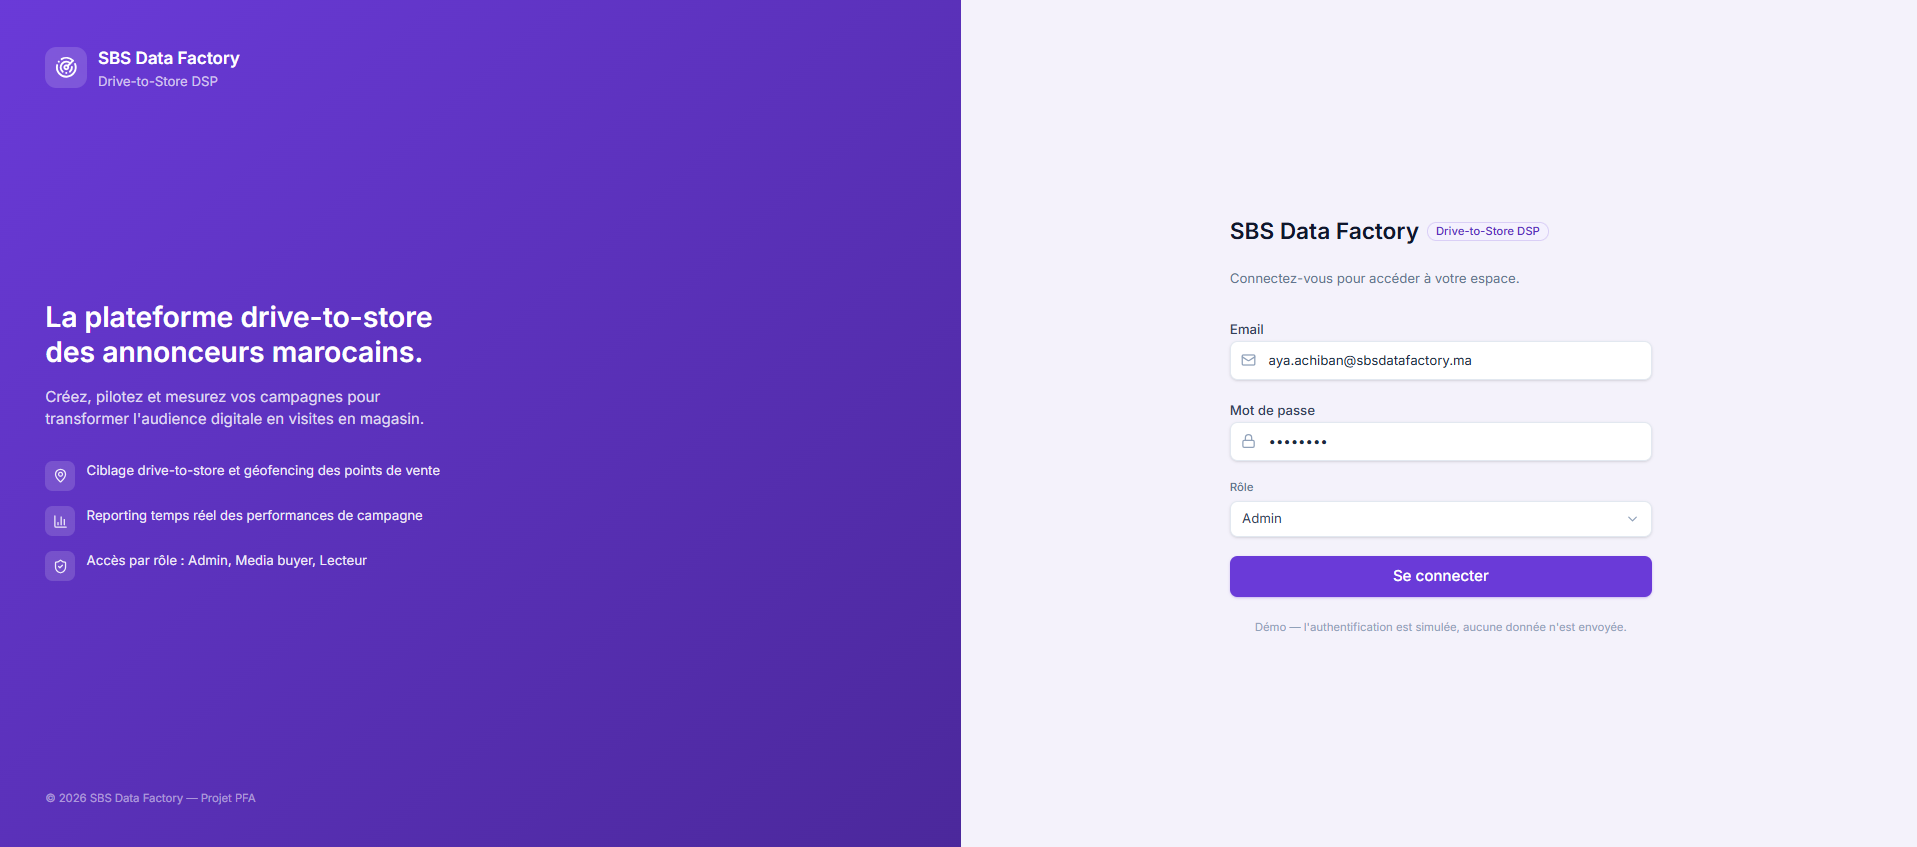
\includegraphics[width=0.92\textwidth]{login.png}
\caption{Interface de connexion}
\label{fig:login}
\end{figure}

%---------------------------------------------------------------------------
\section{Module B --- Tableau de bord}

\subsection*{Objectif}
Donner une vue de synthèse immédiate de l'activité publicitaire.

\subsection*{Fonctionnalités}
\begin{itemize}
  \item quatre \textbf{indicateurs clés} (impressions, clics, budget dépensé,
        campagnes actives) ;
  \item \textbf{graphique de performance} ;
  \item \textbf{tableau des campagnes récentes}.
\end{itemize}

\subsection*{Explication technique}
Les données proviennent d'un endpoint dédié (\texttt{GET
/api/statistics/dashboard}) qui agrège des données \emph{mockées}, prêtes à
être remplacées par de vraies statistiques une fois la base branchée. Les
graphiques utilisent la bibliothèque Recharts.

\begin{figure}[H]
\centering
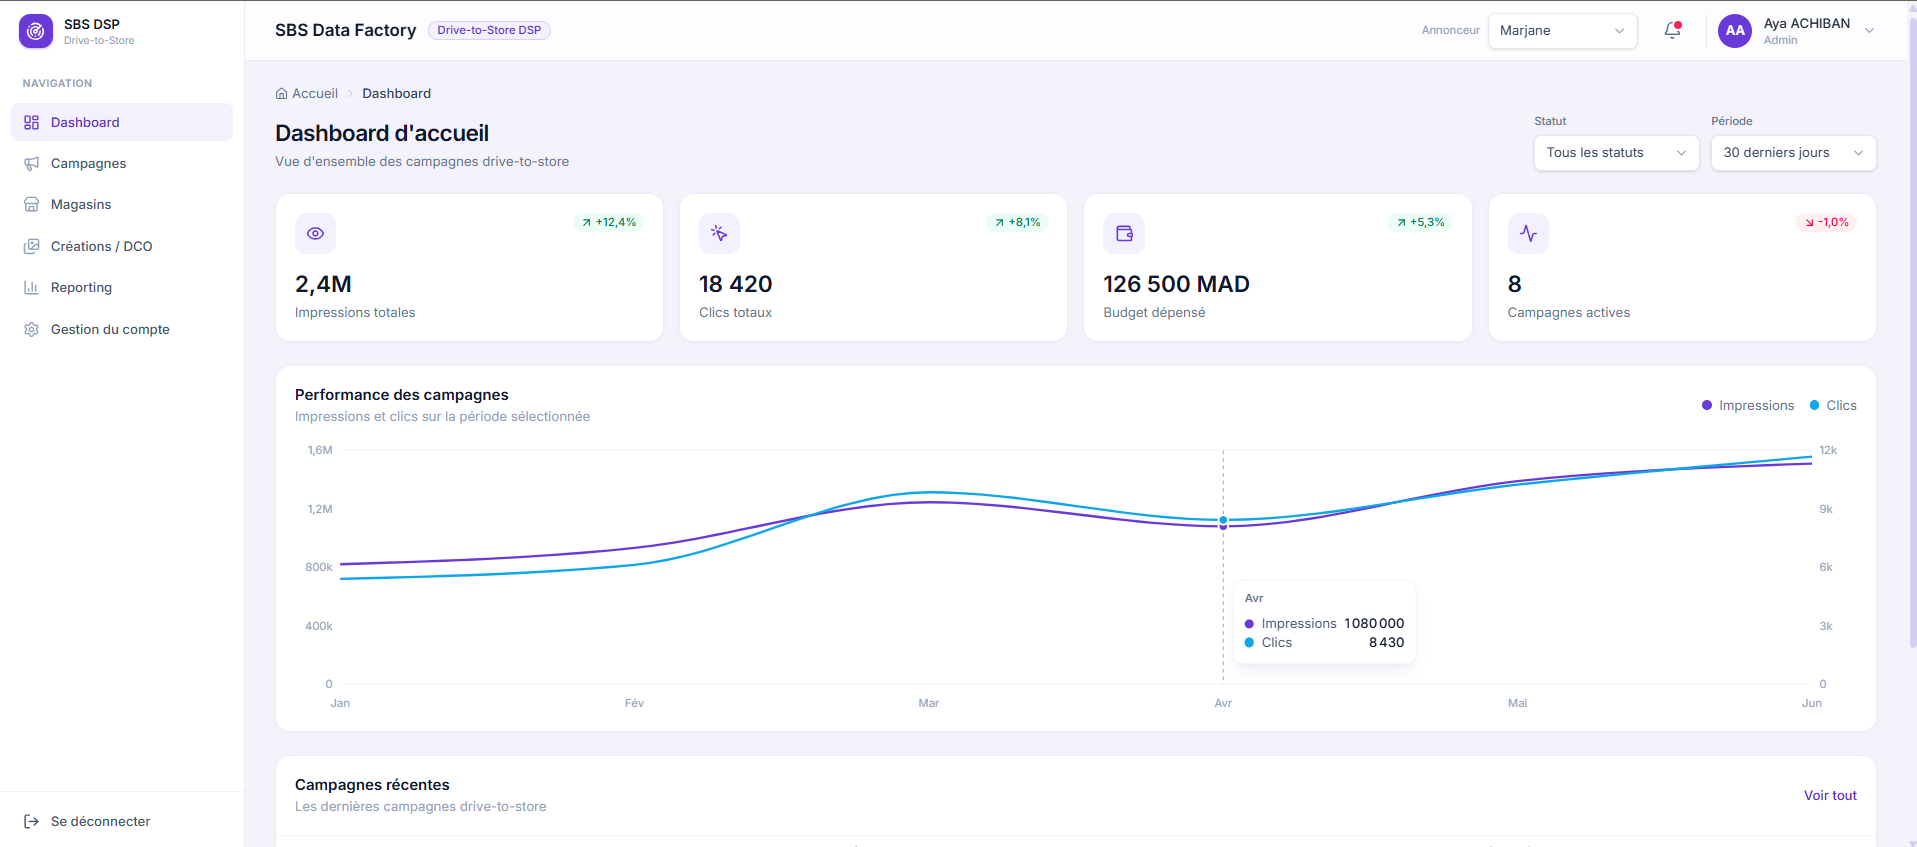
\includegraphics[width=0.92\textwidth]{dashboard.png}
\caption{Tableau de bord principal}
\label{fig:dashboard}
\end{figure}

%---------------------------------------------------------------------------
\section{Module C --- Gestion des campagnes}

\subsection*{Objectif}
Lister les campagnes existantes et les brouillons en cours.

\subsection*{Fonctionnalités}
\begin{itemize}
  \item section \textbf{\og Vos brouillons \fg{}} alimentée par l'API ;
  \item section \textbf{\og Toutes les campagnes \fg{}} présentant des
        campagnes de démonstration (active, en pause, brouillon, terminée) ;
  \item accès direct à l'assistant de création.
\end{itemize}

\subsection*{Explication technique et limite}
La liste des brouillons est \textbf{réellement branchée} au backend
(\texttt{GET /api/campaigns/drafts}). En revanche, la table \og Toutes les
campagnes \fg{} affiche encore des données \emph{mockées} côté frontend : ce
point est signalé en toute transparence et figure parmi les évolutions
possibles.

\begin{figure}[H]
\centering
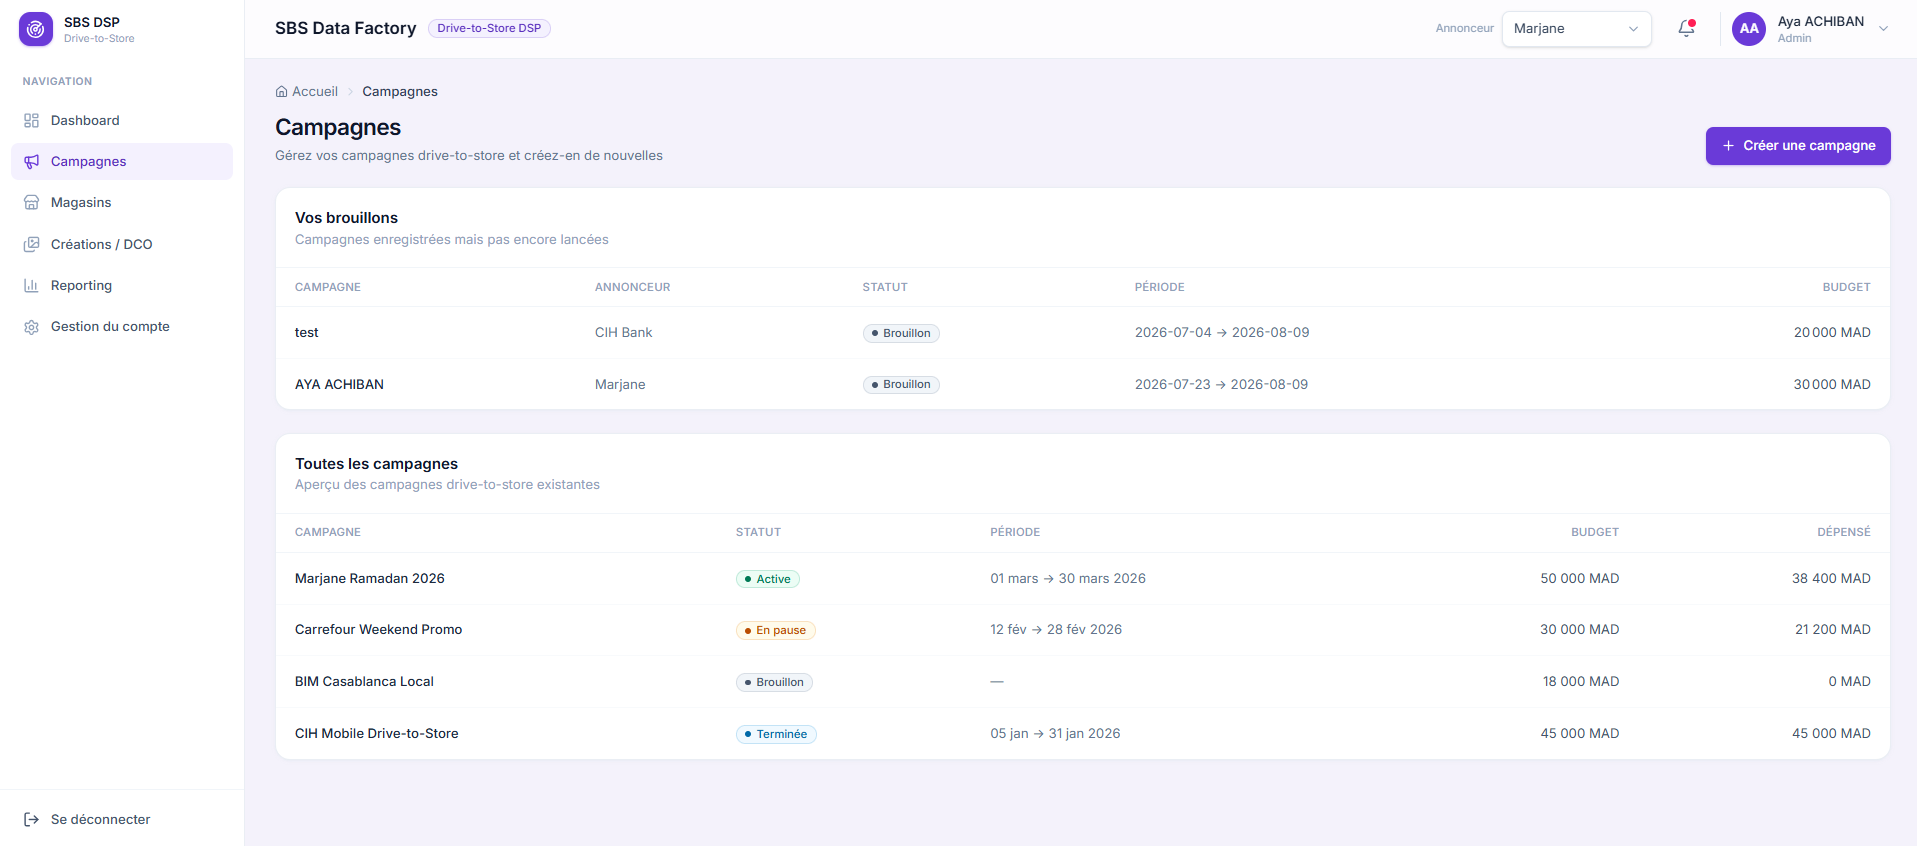
\includegraphics[width=0.92\textwidth]{campagnes.png}
\caption{Liste des campagnes et des brouillons}
\label{fig:campagnes}
\end{figure}

%---------------------------------------------------------------------------
\section{Module D --- Assistant de création de campagne}

\subsection*{Objectif}
Guider l'utilisateur dans la création d'une campagne à travers un parcours
structuré.

\subsection*{Fonctionnalités}
Assistant en \textbf{cinq étapes} : (1) informations générales (nom,
annonceur, objectif, dates, budgets), (2) ciblage technique (appareils,
systèmes d'exploitation, plages horaires), (3) formats publicitaires, (4)
magasins ciblés (voir modules E et F), (5) catégories d'applications et
résumé. À toute étape, l'utilisateur peut \textbf{enregistrer un brouillon},
même incomplet.

\subsection*{Explication technique}
L'assistant s'appuie sur un catalogue d'options servi par l'API
(\texttt{GET /api/campaign-creation/options}), garantissant un vocabulaire
partagé entre frontend et backend. L'enregistrement d'un brouillon
(\texttt{POST /api/campaigns/drafts}) constitue la \textbf{seule donnée
réellement persistée} du prototype ; en cas d'API injoignable, un repli local
(navigateur) évite de bloquer le parcours.

\begin{figure}[H]
\centering
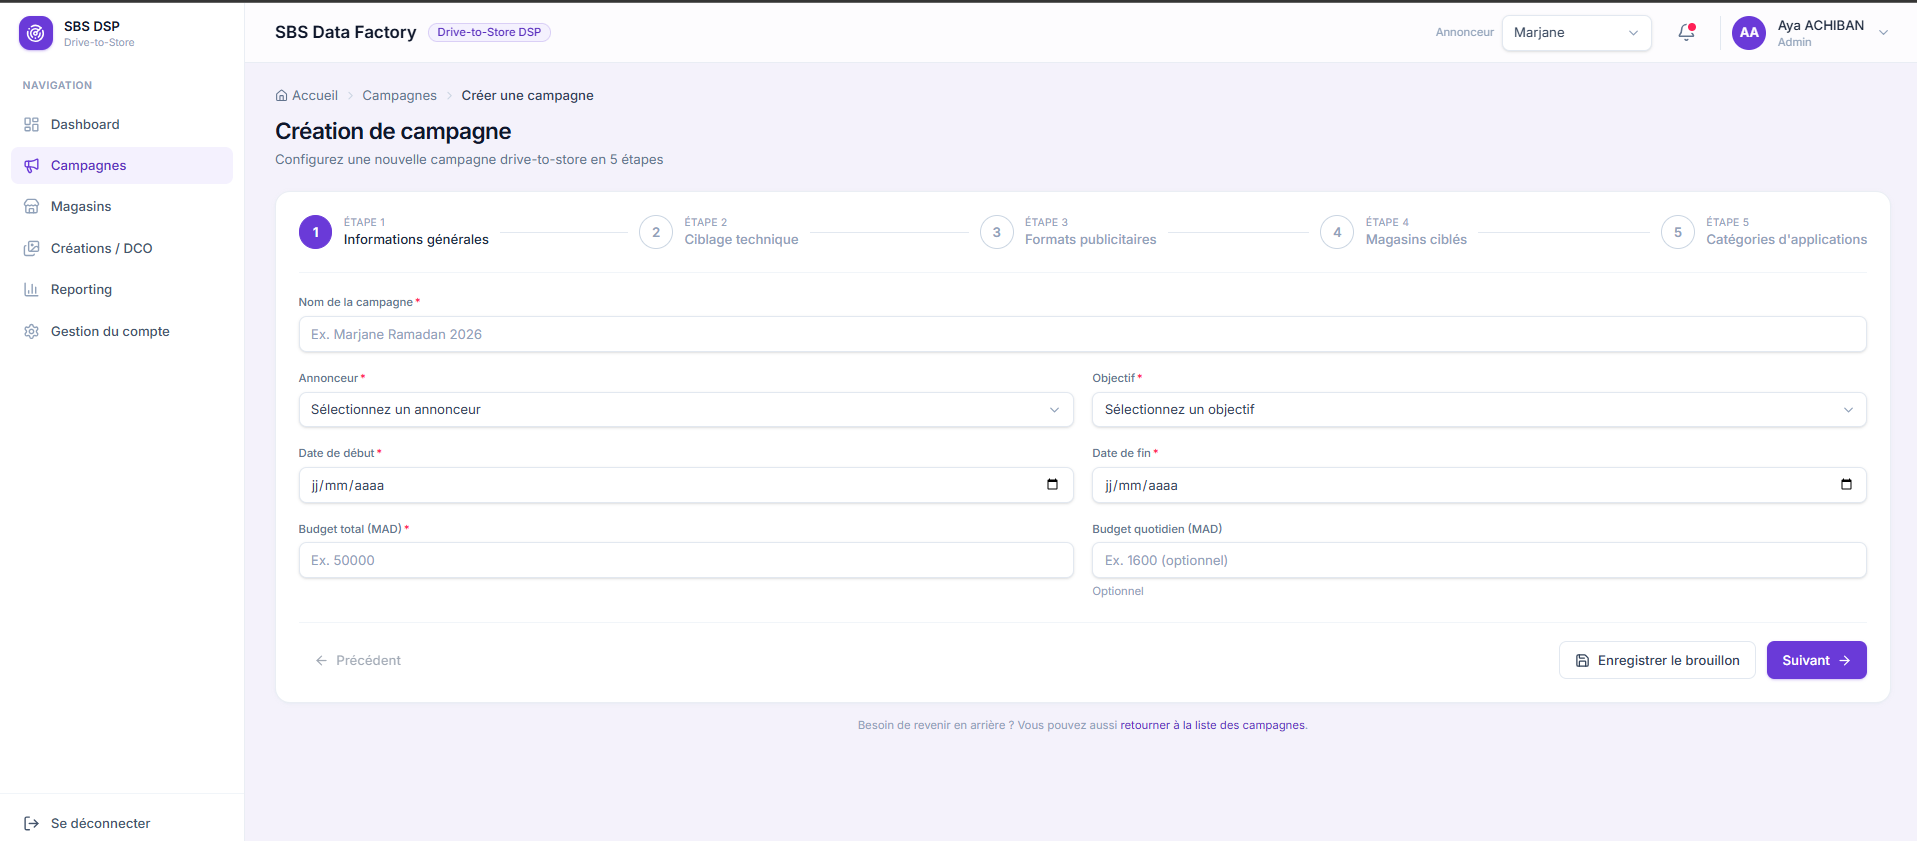
\includegraphics[width=0.92\textwidth]{creation-campagne.png}
\caption{Assistant de création de campagne}
\label{fig:creation}
\end{figure}

%---------------------------------------------------------------------------
\section{Module E --- Import des magasins et validation CSV}

\subsection*{Objectif}
Permettre à l'annonceur d'importer sa base de magasins et en garantir la
qualité avant utilisation.

\subsection*{Fonctionnalités}
\begin{itemize}
  \item import d'un fichier \texttt{.xlsx} ou \texttt{.csv} ;
  \item \textbf{validation ligne par ligne} : colonnes obligatoires,
        coordonnées GPS, format d'URL, détection des doublons ;
  \item affichage du nombre de lignes valides et des erreurs détaillées ;
  \item sélection des magasins à cibler.
\end{itemize}

\subsection*{Explication technique}
La validation est réalisée \textbf{côté serveur}
(\texttt{POST /api/stores/import/preview}) : le fichier est analysé (CSV avec
séparateur \texttt{,} ou \texttt{;}, ou Excel), chaque ligne est contrôlée, et
une erreur explicite est produite par cellule invalide, avec son numéro de
ligne. Aucune donnée n'est persistée à l'étape d'aperçu.

\begin{figure}[H]
\centering
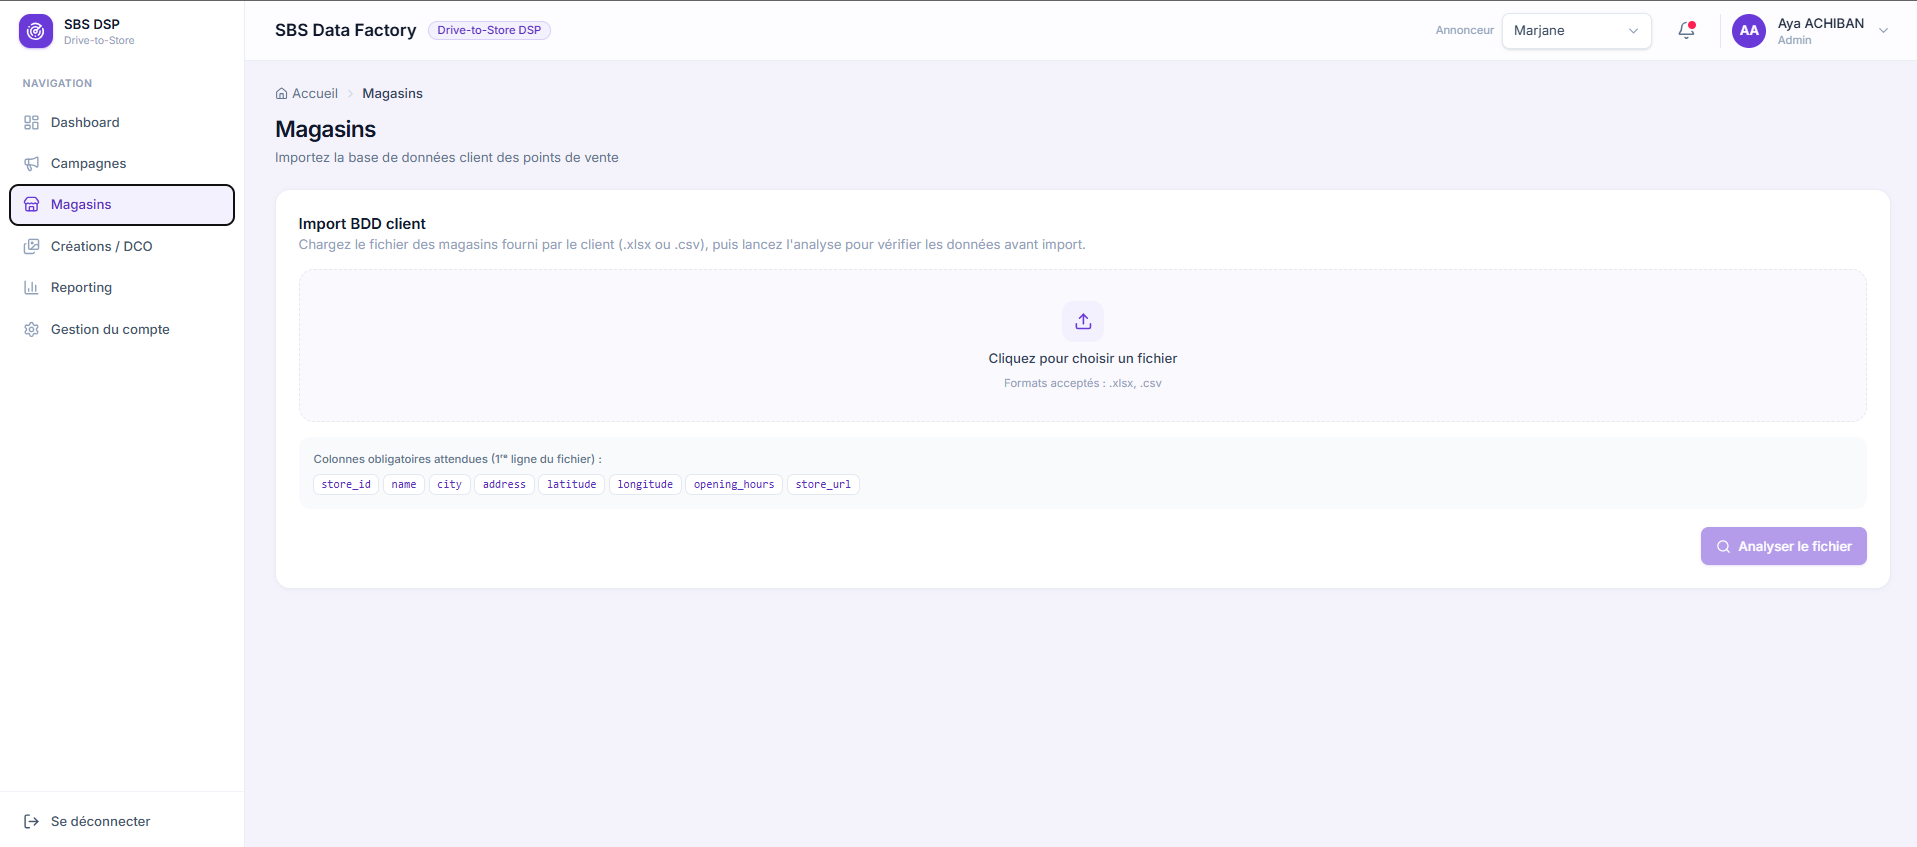
\includegraphics[width=0.92\textwidth]{magasins.png}
\caption{Import et validation de la base de magasins}
\label{fig:magasins}
\end{figure}

%---------------------------------------------------------------------------
\section{Module F --- Géociblage / geofencing}

\subsection*{Objectif}
Définir et visualiser les zones de diffusion autour des magasins sélectionnés.

\subsection*{Fonctionnalités}
\begin{itemize}
  \item carte interactive avec un \textbf{marqueur par magasin} ;
  \item réglage du \textbf{rayon de diffusion} (1 à 20 km, 5 km par défaut) ;
  \item visualisation du rayon par un \textbf{cercle} sur la carte.
\end{itemize}

\subsection*{Explication technique}
La cartographie repose sur \textbf{Leaflet} et les fonds de carte
\textbf{OpenStreetMap} (aucune clé propriétaire requise). Le composant de carte
est \textbf{partagé} entre la page \og Magasins \fg{} et l'étape 4 de
l'assistant, garantissant un comportement identique aux deux endroits.

\begin{figure}[H]
\centering
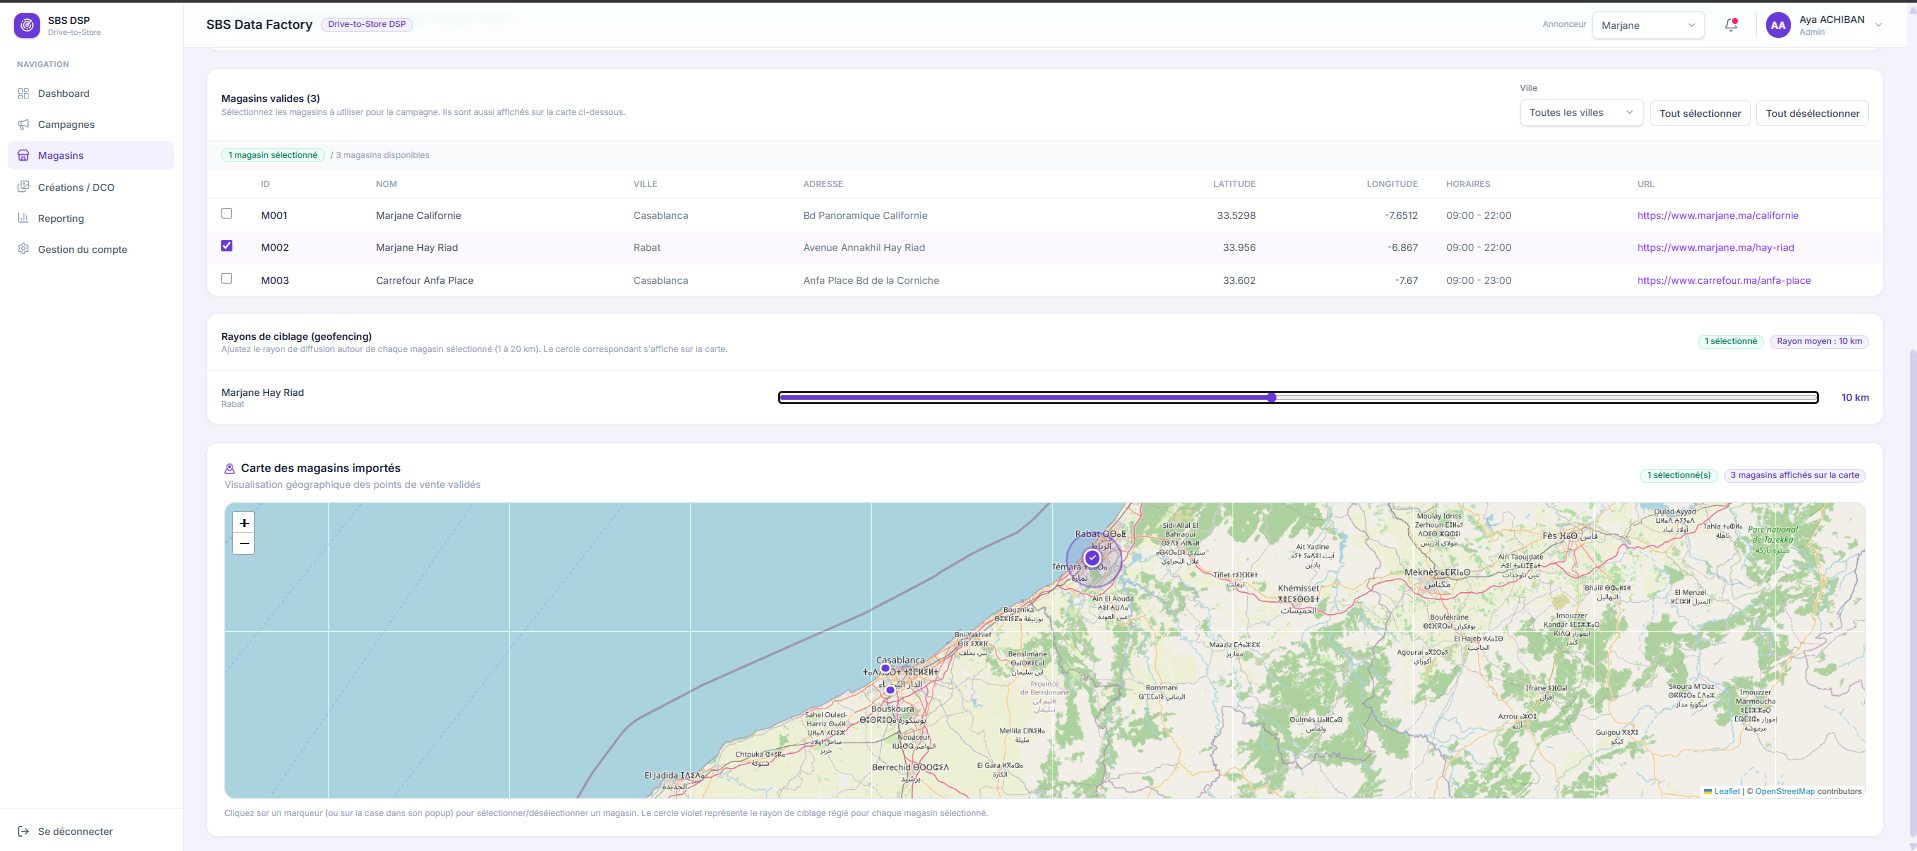
\includegraphics[width=0.92\textwidth]{map-geofencing.png}
\caption{Carte de géociblage (geofencing)}
\label{fig:geofencing}
\end{figure}

%---------------------------------------------------------------------------
\section{Module G --- DCO et landing pages simulées}

\subsection*{Objectif}
Générer automatiquement des créatives et des pages d'atterrissage
personnalisées par magasin.

\subsection*{Fonctionnalités}
\begin{itemize}
  \item upload d'un visuel par format (bannière, pavé, interstitiel) ;
  \item \textbf{génération d'une variante par magasin} intégrant les champs
        dynamiques (nom, ville, adresse, horaires) ;
  \item comparaison de deux magasins et galerie complète des variantes ;
  \item \textbf{\emph{landing pages} simulées} prévisualisables par magasin.
\end{itemize}

\subsection*{Explication technique et limites}
Seules les \textbf{métadonnées} du visuel sont envoyées et enregistrées côté
serveur (\texttt{POST /api/dco/creatives}) : aucun fichier n'est stocké sur
disque. La génération des variantes et des \emph{landing pages} est calculée
\textbf{côté frontend}. Les \emph{landing pages} sont \textbf{entièrement
simulées} (pas de route publique réelle). Enfin, les URL de magasin issues des
données de démonstration sont \textbf{volontairement non cliquables} (texte
informatif), car elles ne pointent pas vers de vraies pages en ligne.

\begin{figure}[H]
\centering
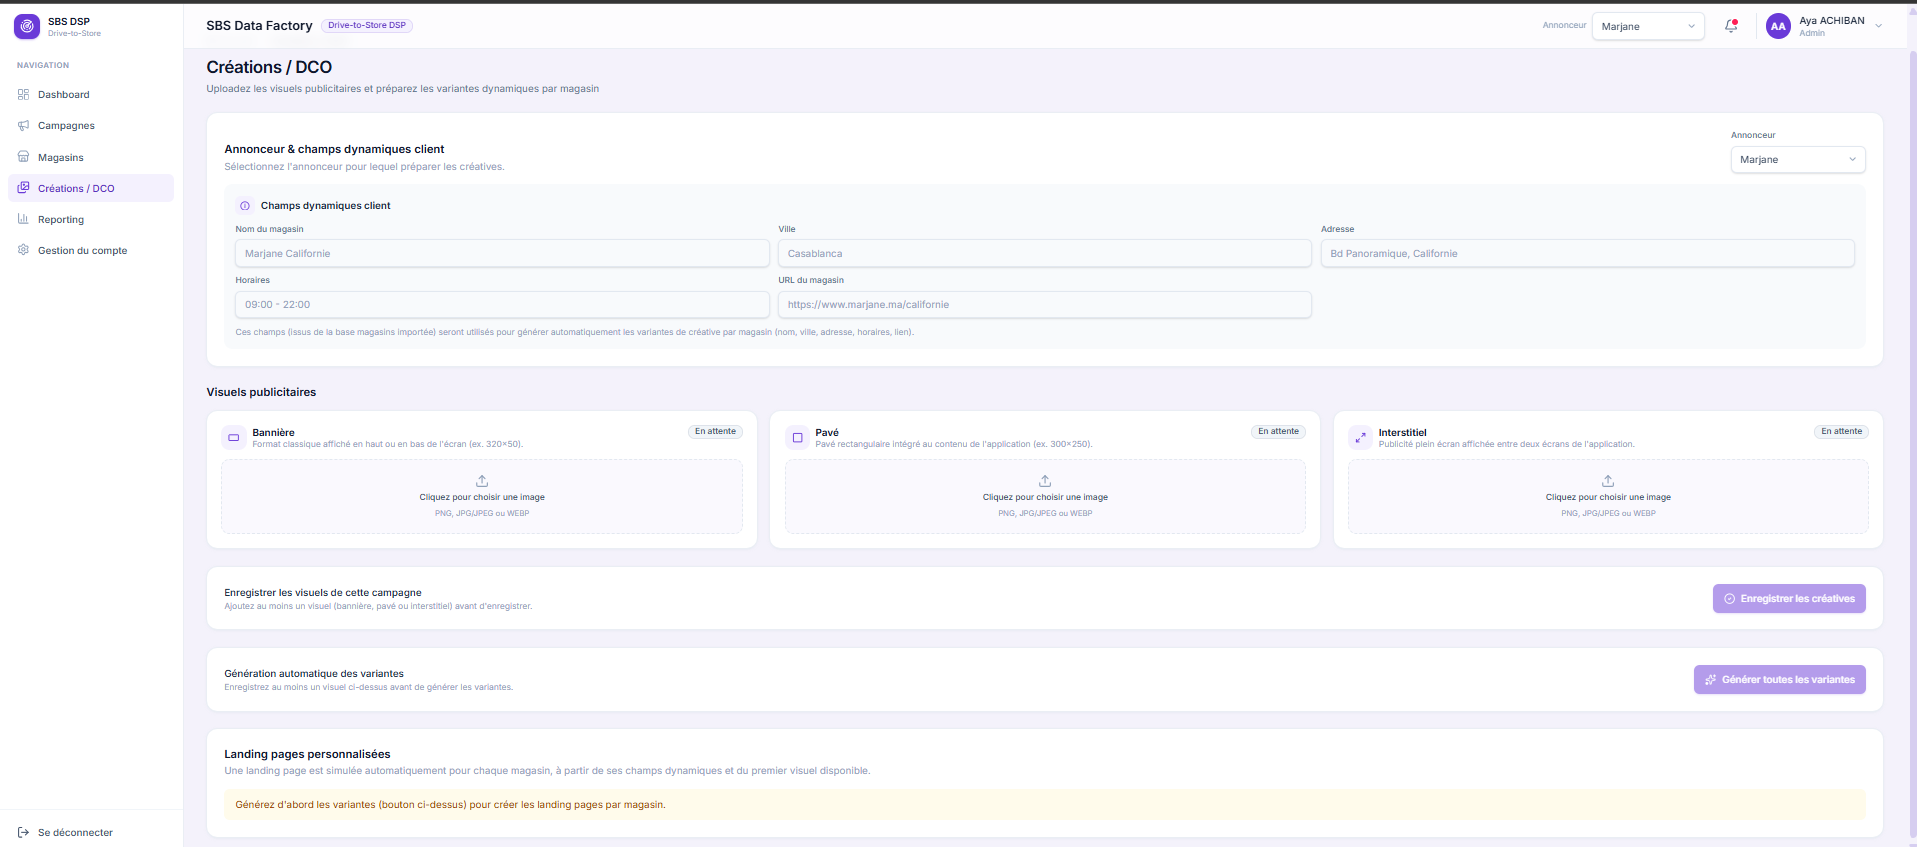
\includegraphics[width=0.92\textwidth]{dco.png}
\caption{Module DCO --- génération de variantes}
\label{fig:dco}
\end{figure}

%---------------------------------------------------------------------------
\section{Module H --- Reporting et export CSV}

\subsection*{Objectif}
Analyser la performance des campagnes selon différents filtres et exporter les
résultats.

\subsection*{Fonctionnalités}
\begin{itemize}
  \item filtres (période, campagne, ville/magasin) ;
  \item \textbf{indicateurs} et \textbf{graphiques} qui se recalculent selon
        les filtres ;
  \item \textbf{carte des zones de diffusion} et \textbf{tableau par magasin}
        triable ;
  \item \textbf{export CSV} compatible Excel.
\end{itemize}

\subsection*{Explication technique et limite}
La liste des magasins et des villes provient de l'endpoint réel
(\texttt{GET /api/stores}). En revanche, les indicateurs de performance sont
\textbf{générés côté frontend} (données de démonstration réalistes), et non
encore agrégés depuis une base. L'export CSV inclut un \textbf{BOM UTF-8} et un
séparateur point-virgule ({\NoAutoSpacing\texttt{;}}), afin de garantir un
affichage correct des accents et des colonnes dans Excel.

\begin{figure}[H]
\centering
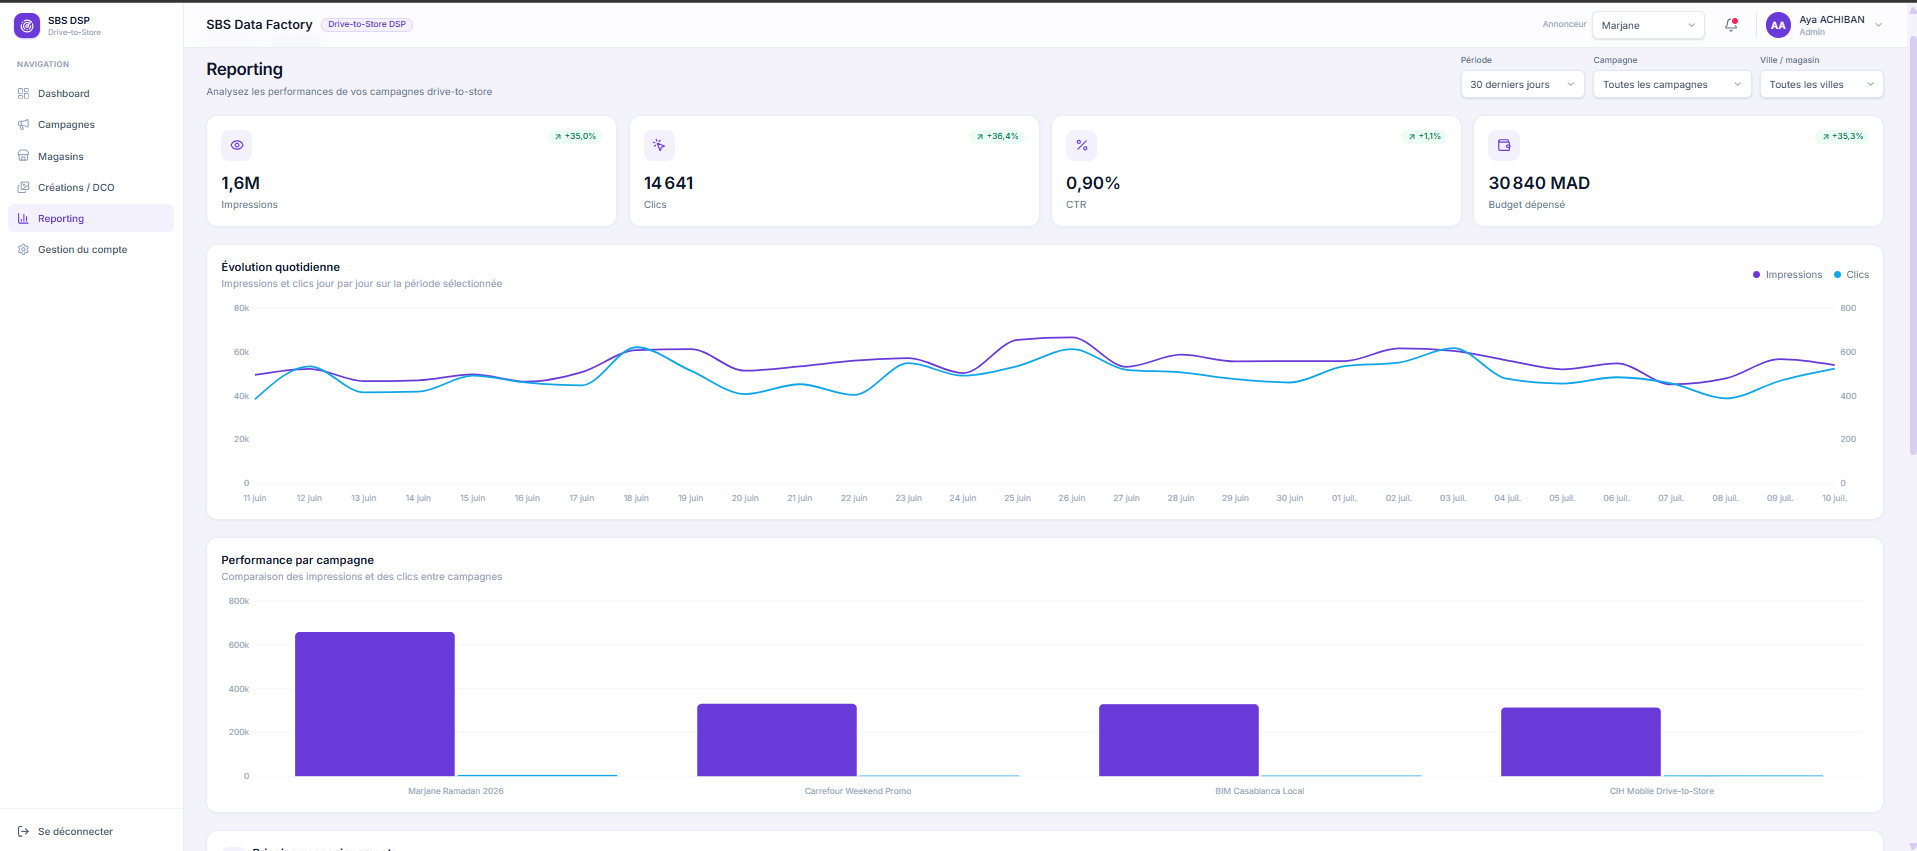
\includegraphics[width=0.92\textwidth]{reporting.png}
\caption{Reporting des performances}
\label{fig:reporting}
\end{figure}

%---------------------------------------------------------------------------
\section{Module I --- Gestion du compte}

\subsection*{Objectif}
Administrer les annonceurs, les utilisateurs et les paramètres du compte.

\subsection*{Fonctionnalités}
\begin{itemize}
  \item onglet \textbf{Annonceurs} : recherche, filtre, fiche détaillée,
        modification ;
  \item onglet \textbf{Utilisateurs} : recherche, filtre par rôle, ajout,
        modification, activation/désactivation ;
  \item onglet \textbf{Paramètres} : devise, fuseau horaire, langue, e-mail de
        notification, activation du suivi.
\end{itemize}

\subsection*{Explication technique}
Le module est \textbf{entièrement branché sur l'API}
(\texttt{/api/advertisers}, \texttt{/api/users}, \texttt{/api/account-settings}),
avec des erreurs HTTP explicites (404 pour un identifiant inconnu, 409 pour un
e-mail déjà utilisé, 422 pour un champ invalide). L'\textbf{édition} est
réservée au rôle Admin ; les autres rôles accèdent en lecture seule.

\begin{figure}[H]
\centering
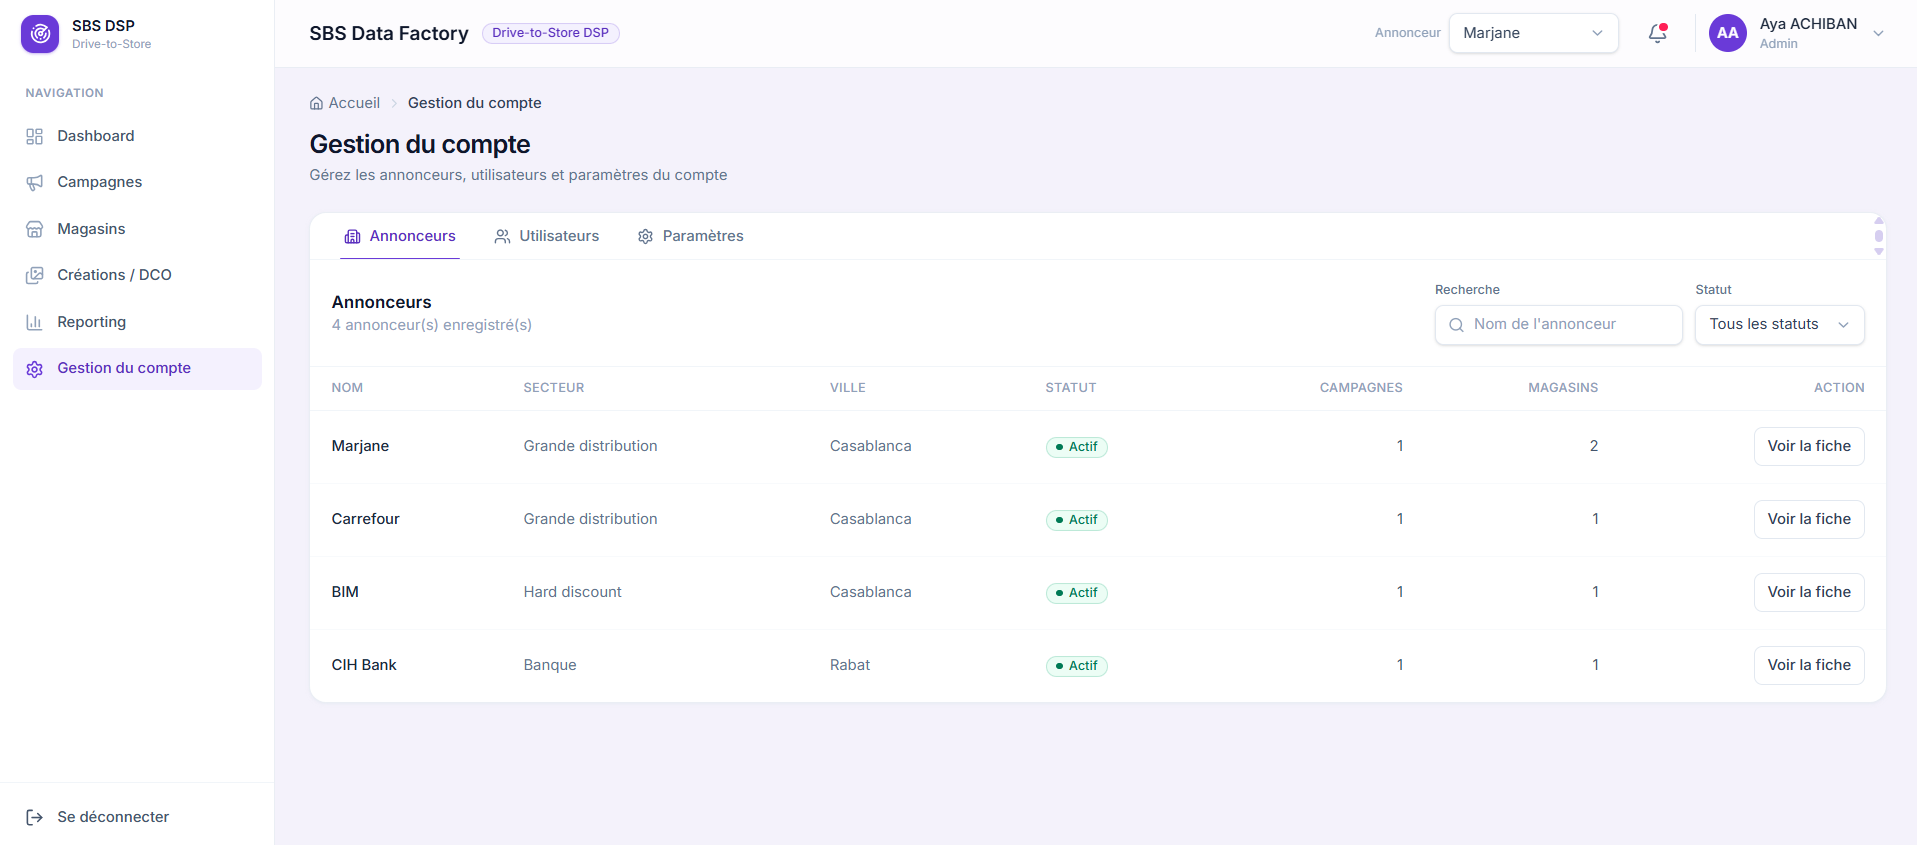
\includegraphics[width=0.92\textwidth]{gestion-compte.png}
\caption{Gestion du compte (annonceurs, utilisateurs, paramètres)}
\label{fig:compte}
\end{figure}

%---------------------------------------------------------------------------
\section{Module J --- Backend FastAPI et Swagger}

\subsection*{Objectif}
Exposer une API REST claire, validée et documentée.

\subsection*{Fonctionnalités}
\begin{itemize}
  \item \textbf{24 endpoints} REST regroupés par ressource ;
  \item validation des données par Pydantic et erreurs HTTP explicites ;
  \item documentation \textbf{Swagger/OpenAPI} interactive et testable.
\end{itemize}

\subsection*{Explication technique}
FastAPI génère automatiquement la documentation OpenAPI, accessible à
l'adresse \texttt{/docs}. Chaque endpoint y est décrit et peut être exécuté
directement depuis l'interface. La figure~\ref{fig:swagger} présente la vue
d'ensemble de l'API, et la figure~\ref{fig:swaggerhealth} illustre le test de
l'endpoint de santé.

\begin{figure}[H]
\centering
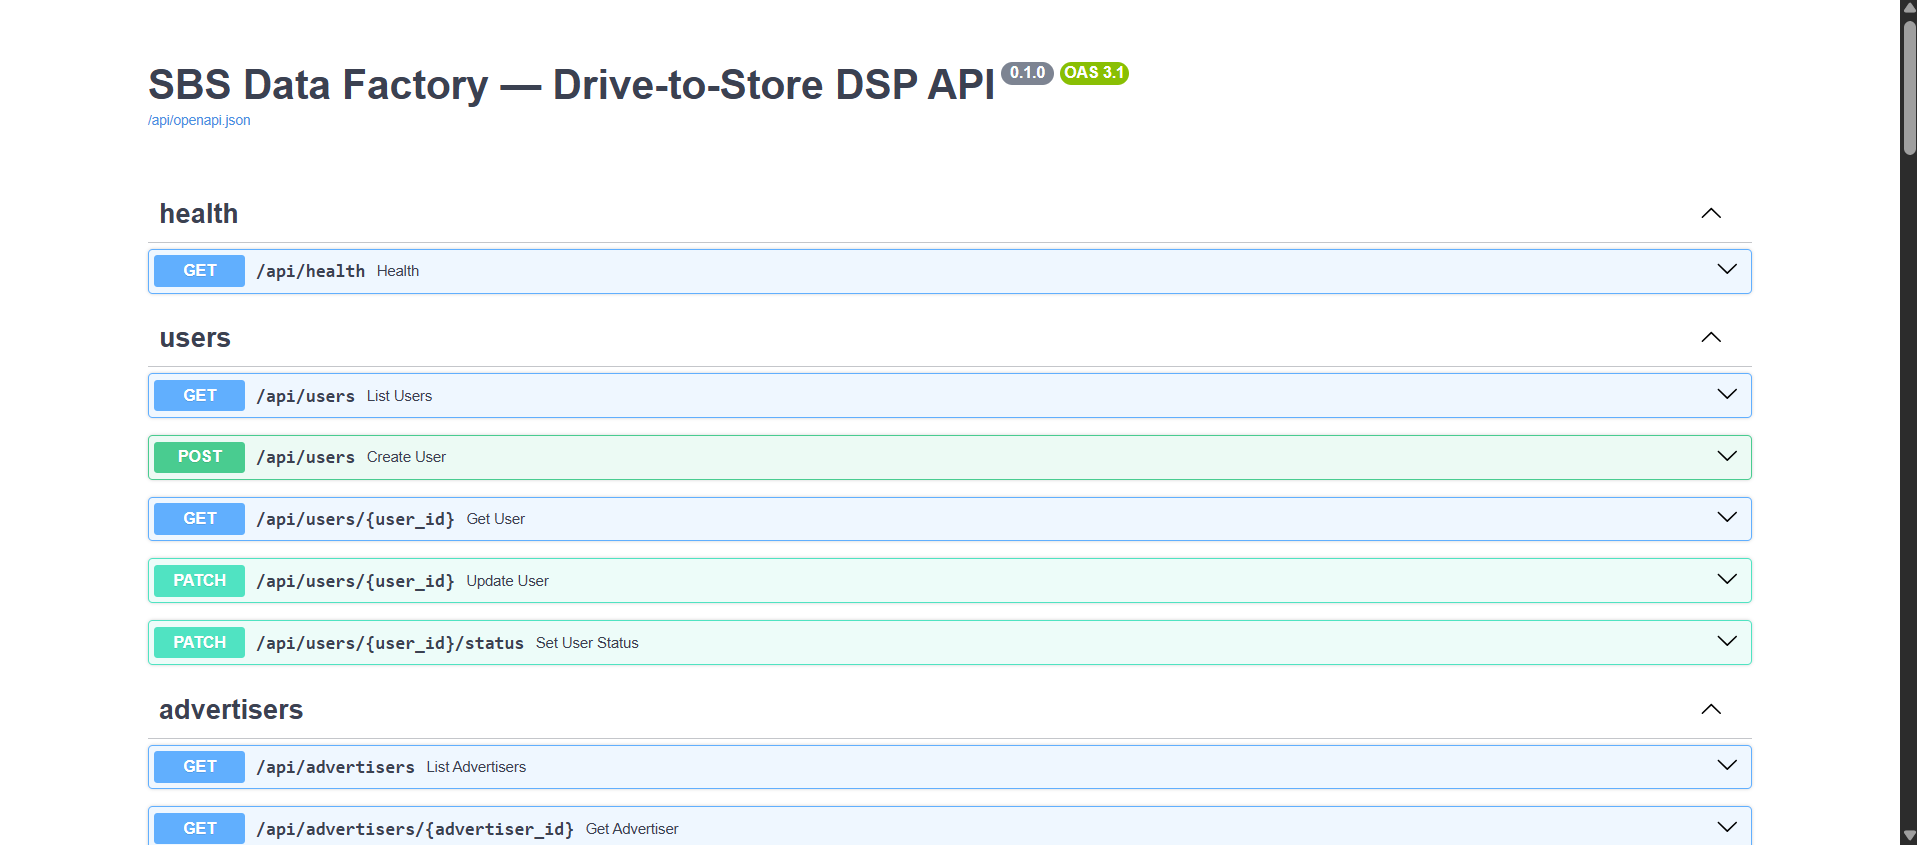
\includegraphics[width=0.92\textwidth]{swagger-api.png}
\caption{Documentation Swagger de l'API}
\label{fig:swagger}
\end{figure}

\begin{figure}[H]
\centering
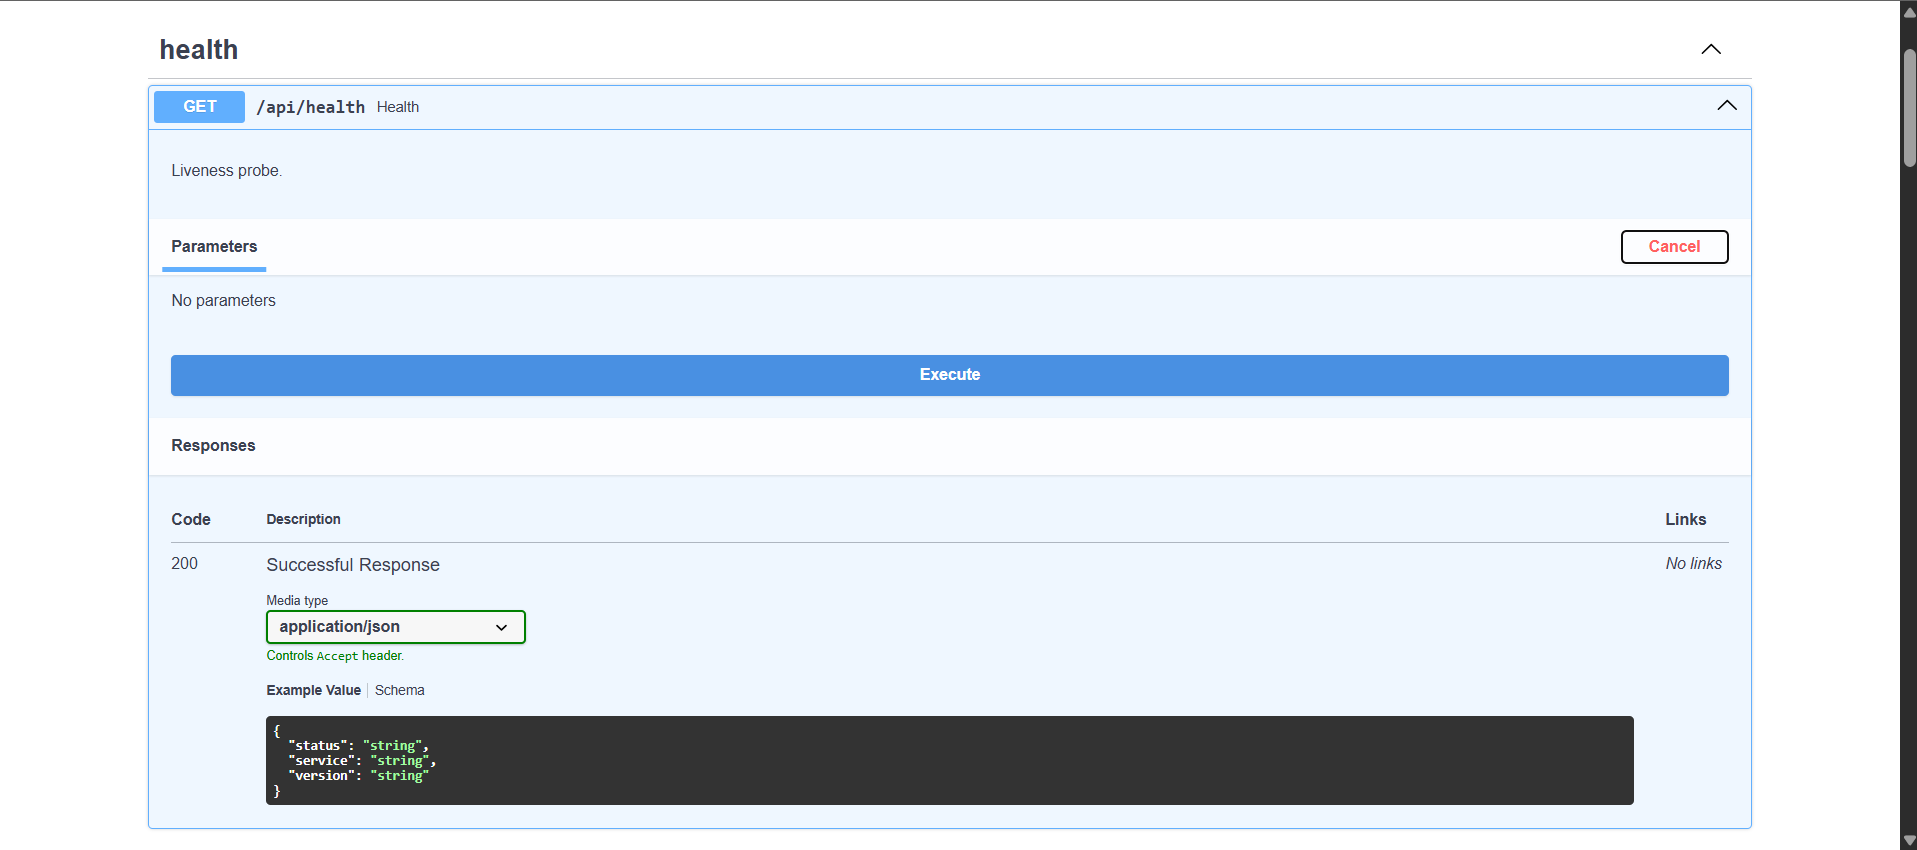
\includegraphics[width=0.92\textwidth]{swagger-health-test.png}
\caption{Test de l'endpoint \texttt{/api/health} depuis Swagger}
\label{fig:swaggerhealth}
\end{figure}

%---------------------------------------------------------------------------
\section{Module K --- GitHub et documentation}

\subsection*{Objectif}
Assurer un versionnement rigoureux et une documentation exploitable du projet.

\subsection*{Fonctionnalités}
\begin{itemize}
  \item dépôt GitHub structuré (\texttt{frontend/}, \texttt{backend/},
        \texttt{database/}, \texttt{docs/}) ;
  \item flux par \textbf{branches} et \textbf{\emph{pull requests}} ;
  \item documentation continue (technique, schéma de données, scénario et
        checklist de démonstration, journal d'avancement, livraison finale).
\end{itemize}

\subsection*{Explication technique}
Chaque incrément a été développé sur une branche dédiée puis intégré par
\emph{pull request}, ce qui conserve un historique lisible et réversible. La
figure~\ref{fig:github} présente le dépôt du projet.

\begin{figure}[H]
\centering
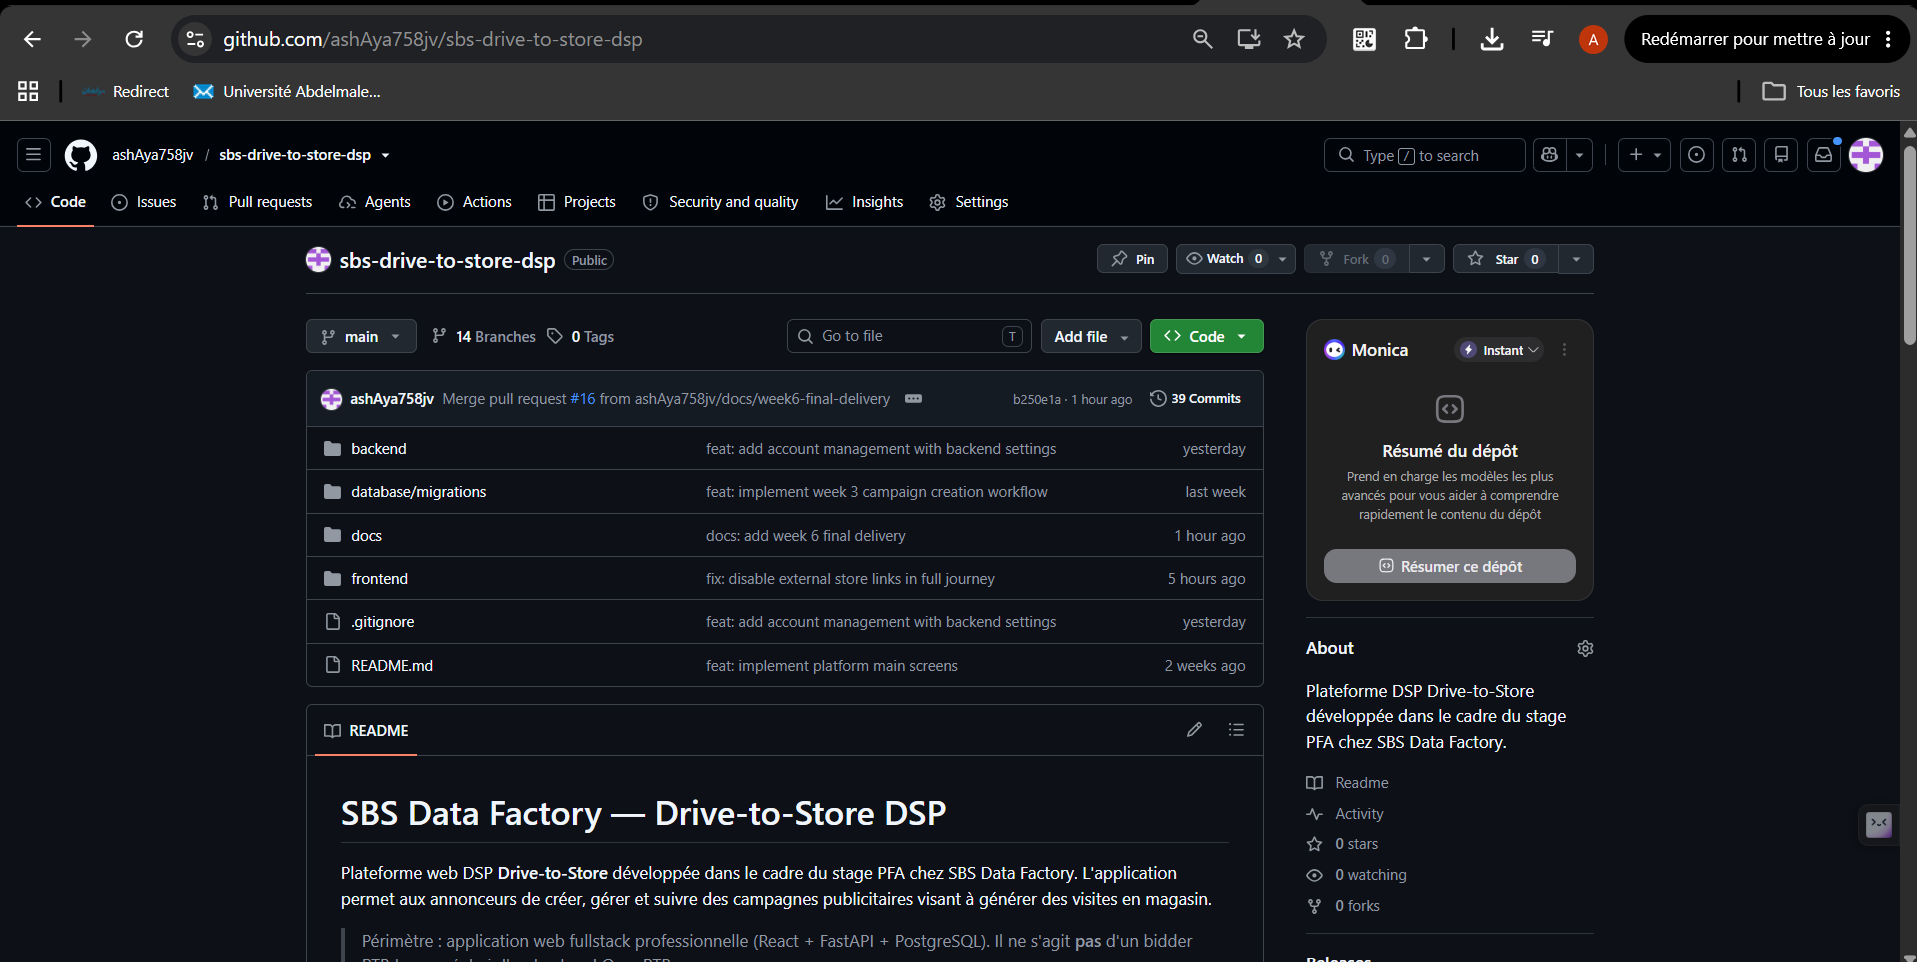
\includegraphics[width=0.92\textwidth]{github-repository.png}
\caption{Dépôt GitHub du projet}
\label{fig:github}
\end{figure}

%============================ TESTS ET VALIDATION ===========================
\chapter{Tests et validation}

\section{Stratégie de validation}

La validation du prototype a été réalisée de manière \textbf{manuelle et
systématique}, module par module, puis de bout en bout. En l'absence de tests
automatisés à ce stade (voir limites), l'accent a été mis sur des vérifications
reproductibles : build, contrôle de santé de l'API, exécution des endpoints via
Swagger, et parcours utilisateur complet dans le navigateur.

\section{Vérifications réalisées}

Le tableau~\ref{tab:tests} récapitule les principales vérifications et leur
résultat.

\begin{table}[H]
\centering
\caption{Synthèse des tests et validations}
\label{tab:tests}
\small
\begin{tabularx}{\textwidth}{@{}p{5.2cm}L p{2cm}@{}}
\toprule
\textbf{Vérification} & \textbf{Détail} & \textbf{Résultat} \\
\midrule
Build du frontend & \texttt{npm run build} sans erreur & Validé \\
Analyse statique & \texttt{npm run lint} sans avertissement & Validé \\
Santé du backend & \texttt{GET /api/health} renvoie le statut \texttt{ok} & Validé \\
API Swagger & Endpoints listés et exécutables depuis \texttt{/docs} & Validé \\
Navigation & Menu adapté au rôle, fil d'Ariane correct & Validé \\
Connexion / déconnexion & Ouverture et fermeture de session & Validé \\
Routes protégées & Redirection si non authentifié ou rôle non autorisé & Validé \\
Création de campagne & Parcours complet et enregistrement du brouillon & Validé \\
Import des magasins & Validation des lignes et détection d'erreurs & Validé \\
Carte de geofencing & Marqueurs et rayons affichés correctement & Validé \\
Génération DCO & Variantes par magasin et \emph{landing pages} simulées & Validé \\
Filtres de reporting & Indicateurs et graphiques recalculés & Validé \\
Export CSV & Fichier lisible dans Excel (accents, colonnes) & Validé \\
Paramètres du compte & Mise à jour via \texttt{PATCH /api/account-settings} & Validé \\
Validation fonctionnelle finale & Parcours de bout en bout cohérent & Validé \\
\bottomrule
\end{tabularx}
\end{table}

\section{Contrôle de non-régression}

À chaque nouvelle étape, les modules précédemment validés ont été parcourus
de nouveau afin de détecter d'éventuelles régressions. Cette vigilance a
notamment permis de corriger, lors de l'intégration de bout en bout, des
détails de navigation (par exemple des liens externes de démonstration rendus
volontairement non cliquables pour éviter d'ouvrir des pages inexistantes).

\section{Cas d'erreur couverts}

Au-delà des cas nominaux, plusieurs cas d'erreur ont été vérifiés côté API :
identifiant inconnu (404), e-mail déjà utilisé lors de la création d'un
utilisateur (409), champ invalide ou manquant (422), fichier d'import au
format non supporté ou illisible (400). Ces réponses sont explicites et
exploitées par l'interface pour afficher des messages clairs.

\section{Limite de la démarche}

La validation reste \textbf{manuelle} : elle ne remplace pas une suite de
\textbf{tests automatisés} (unitaires et de bout en bout), dont la mise en
place figure parmi les perspectives du projet. La procédure de validation est
toutefois documentée et reproductible (voir le chapitre suivant).

%======================= DOCUMENTATION ET LIVRAISON =========================
\chapter{Documentation et livraison}

\section{Une documentation produite en continu}

La documentation a accompagné le développement à chaque étape, plutôt que
d'être produite en fin de projet. Elle est regroupée dans le dossier
\texttt{docs/} du dépôt et couvre à la fois les aspects techniques,
fonctionnels et organisationnels. Le tableau~\ref{tab:docs} en présente les
principaux documents.

\begin{table}[H]
\centering
\caption{Documents de référence du dépôt}
\label{tab:docs}
\small
% Noms de fichiers composés avec \path : coupure autorisée aux tirets et
% points, ce qui évite tout débordement dans la colonne voisine.
\begin{tabularx}{\textwidth}{@{}p{6.2cm}L@{}}
\toprule
\textbf{Document} & \textbf{Contenu} \\
\midrule
\path{documentation-technique.md} & Architecture, structure des dossiers, installation, 24~endpoints avec exemples, schéma des entités, limites, pistes de déploiement. \\
\path{schema-base-de-donnees.md} & Schéma PostgreSQL cible (tables, contraintes, relations). \\
\path{scenario-demonstration-finale.md} & Script de démonstration en neuf étapes, texte oral et points techniques. \\
\path{checklist-demonstration-finale.md} & Checklists avant, pendant et après la démonstration ; erreurs courantes et solutions. \\
\path{livraison-finale-semaine-6.md} & Document de synthèse de livraison, prêt à être remis à l'encadrante. \\
\path{etat-avancement-semaine-6.md} & Journal détaillé, jour par jour, de la semaine~6. \\
\bottomrule
\end{tabularx}
\end{table}

\section{Documentation de l'API}

L'API est documentée de deux manières complémentaires : de façon
\textbf{interactive} via \textbf{Swagger/OpenAPI} (accessible à \texttt{/docs},
avec exécution directe des endpoints), et de façon \textbf{écrite} dans
\texttt{documentation-technique.md}, qui recense l'ensemble des endpoints avec
leur méthode, leur rôle et un exemple de réponse. Ce double niveau garantit
qu'un développeur reprenant le projet dispose à la fois d'une référence testable
et d'une référence rédigée.

\section{Préparation de la démonstration}

En vue de la présentation finale, deux documents dédiés ont été produits :

\begin{itemize}
  \item un \textbf{scénario de démonstration} détaillant, en neuf étapes, le
        parcours exact à montrer, avec pour chaque étape un texte oral court et
        les points techniques à mentionner ;
  \item une \textbf{checklist de démonstration} regroupant les vérifications
        avant, pendant et après la démo, un tableau des incidents courants
        (backend non lancé, port occupé, page blanche, cache navigateur,
        export CSV, erreur API) avec leur solution rapide, ainsi qu'un ordre
        recommandé de captures d'écran pour préparer des supports.
\end{itemize}

\section{Livraison finale}

La livraison finale prend la forme d'un document de synthèse
(\texttt{livraison-finale-semaine-6.md}) reprenant le périmètre livré, les
modules, l'état technique, les commandes de lancement, les endpoints
principaux, les limites honnêtes et les prochaines améliorations. L'ensemble du
code et de la documentation est versionné sur \textbf{GitHub}, chaque incrément
ayant été intégré par \emph{pull request}, ce qui rend la livraison
\textbf{traçable} et \textbf{reproductible}.

%========================= LIMITES ET PERSPECTIVES ==========================
\chapter{Limites et perspectives}

\section{Limites actuelles du prototype}

Par souci de transparence, les limites du livrable sont énoncées clairement.
Elles découlent de choix assumés, cohérents avec la nature \textbf{prototype}
du projet.

\begin{itemize}
  \item \textbf{Prototype local} : l'application n'est pas déployée en
        production ; elle s'exécute en environnement de développement.
  \item \textbf{Données majoritairement mockées / en mémoire} :
        utilisateurs, annonceurs, magasins, campagnes existantes, créatives et
        paramètres de compte sont réinitialisés à chaque redémarrage du
        backend. Seuls les \textbf{brouillons de campagne} sont réellement
        persistés.
  \item \textbf{PostgreSQL non branché en production} : les modèles et les
        migrations existent et sont prêts, mais la base n'est pas connectée
        par défaut.
  \item \textbf{Authentification non \og production \fg{}} : l'authentification
        est \emph{simulée} (aucun mot de passe vérifié, aucun jeton de session
        réel) ; le contrôle d'accès n'est appliqué que côté frontend.
  \item \textbf{DCO simulé} : aucun fichier de créative n'est réellement stocké
        (métadonnées uniquement), et les \emph{landing pages} sont entièrement
        \textbf{simulées} (pas de route publique réelle).
  \item \textbf{Reporting sur données de démonstration} : les indicateurs et
        graphiques sont générés côté frontend, non encore agrégés depuis une
        base réelle.
  \item \textbf{Absence de connexion à un réseau publicitaire réel} : aucune
        intégration DSP / réseau d'annonces (RTB, OpenRTB) n'est en place ;
        ce n'était pas l'objet du projet.
  \item \textbf{Pas de tests automatisés} : la validation reste manuelle et
        documentée.
  \item \textbf{URL de magasin non cliquables} : les URL des données de
        démonstration sont volontairement rendues non cliquables pour éviter
        d'ouvrir des pages inexistantes.
\end{itemize}

\section{Perspectives d'évolution}

Le prototype a été conçu pour \textbf{faciliter son évolution}. Les axes
d'amélioration suivants découlent directement de l'état actuel :

\begin{enumerate}[label=\textbf{\arabic*.}]
  \item \textbf{Intégration complète de PostgreSQL} : renseigner la connexion,
        appliquer les migrations SQL existantes et remplacer progressivement
        les services \emph{mockés} par de vraies requêtes.
  \item \textbf{Authentification et autorisation réelles} : mots de passe
        hachés, session ou jeton (JWT), contrôle d'accès vérifié côté API.
  \item \textbf{Persistance réelle des créatives DCO} et des variantes
        générées (stockage de fichiers).
  \item \textbf{Reporting sur données réelles} : agrégation de vraies
        statistiques depuis la base.
  \item \textbf{Dockerisation} de l'application (frontend, backend, base) pour
        un environnement reproductible.
  \item \textbf{Intégration continue (CI/CD)} : build, tests et déploiement
        automatisés.
  \item \textbf{Tests automatisés} : unitaires côté backend et de bout en bout
        côté frontend.
  \item \textbf{Déploiement en production} : hébergement du frontend statique
        et du backend ASGI, avec une stratégie de sauvegarde de la base.
  \item \textbf{Moteur DCO réel} et \textbf{intégration à un réseau
        publicitaire / DSP} pour la diffusion effective des campagnes.
  \item \textbf{Analytique avancée} : attribution des visites en magasin,
        indicateurs de fréquentation, tableaux de bord enrichis.
\end{enumerate}

Ces perspectives dessinent une trajectoire réaliste, du \textbf{prototype
validé} vers une \textbf{version de production}, en tirant parti de
l'architecture déjà mise en place.

%============================== CONCLUSION ==================================
\chapter{Conclusion générale}

Ce projet de fin d'année a permis de concevoir et de développer, pour SBS Data
Factory, un \textbf{prototype fonctionnel de bout en bout} d'une plateforme web
de gestion de campagnes publicitaires \emph{drive-to-store}. Le livrable couvre
l'intégralité du parcours métier visé : connexion et navigation protégée par
rôle, tableau de bord, gestion et création de campagnes, import et validation
de la base de magasins, ciblage géographique sur carte, génération de créatives
dynamiques et de \emph{landing pages} personnalisées, reporting complet avec
export, et administration du compte --- le tout appuyé sur une API backend
\textbf{documentée et testable} (24 endpoints, Swagger interactif).

Sur le plan technique, le projet a mis en \oe uvre une \textbf{architecture
fullstack claire} (React/Vite et FastAPI), une \textbf{séparation nette des
responsabilités}, une \textbf{cartographie libre} (Leaflet/OpenStreetMap) et un
\textbf{flux de versionnement rigoureux} (branches et \emph{pull requests}).
La base de données PostgreSQL a été \textbf{préparée} (modèles et migrations)
sans bloquer le fonctionnement du prototype, et la documentation a été produite
\textbf{en continu}.

Le choix, assumé et documenté, de s'appuyer sur des \textbf{données simulées} et
une \textbf{authentification simulée} (à l'exception des brouillons de campagne
réellement persistés) a permis de \textbf{valider l'ensemble des parcours
utilisateur} avant d'investir dans le branchement d'une base réelle et d'une
sécurité de niveau production. Les limites correspondantes ont été énoncées avec
transparence, et une trajectoire d'évolution claire a été tracée.

Au-delà du résultat livré, ce stage a été une expérience formatrice sur
plusieurs plans : la \textbf{conduite itérative} d'un projet réel, la
\textbf{maîtrise d'une stack moderne} (React, FastAPI, OpenAPI, Leaflet), la
\textbf{discipline de versionnement} et de documentation, et la capacité à
faire des \textbf{choix d'ingénierie pragmatiques} en distinguant clairement ce
qui est réel de ce qui est simulé. Ces compétences, à la croisée du
développement web et du marketing digital, constituent un socle solide pour la
suite du parcours, et le prototype réalisé offre une base saine et évolutive
pour de futurs développements au sein de SBS Data Factory.


%--------------------------- Bibliographie ------------------------------------
%========================= BIBLIOGRAPHIE / WEBOGRAPHIE ======================
% Chapitre non numéroté : une seule entrée dans la table des matières (via
% \addcontentsline) et marques d'en-tête posées explicitement. La liste est
% composée manuellement (pas d'environnement thebibliography) afin d'éviter
% le double titre « Bibliographie » et l'en-tête erroné sur les pages
% suivantes que cet environnement génère dans la classe report.
\chapter*{Bibliographie et webographie}
\addcontentsline{toc}{chapter}{Bibliographie et webographie}
\markboth{Bibliographie et webographie}{Bibliographie et webographie}

Les références ci-dessous renvoient aux documentations officielles des
technologies utilisées dans le projet ; il s'agit d'une webographie, aucune
source académique n'étant nécessaire au sujet traité. L'ensemble de ces
ressources en ligne a été consulté le 11~juillet~2026. Une version
\texttt{BibTeX} de ces références est fournie dans le fichier
\texttt{references.bib} accompagnant ce rapport.

\begin{enumerate}[label={[\arabic*]}, leftmargin=1.5cm, itemsep=4pt]
  \item React --- \emph{Documentation officielle}.
        \url{https://react.dev/}
  \item Vite --- \emph{Next Generation Frontend Tooling}.
        \url{https://vitejs.dev/}
  \item React Router --- \emph{Documentation officielle}.
        \url{https://reactrouter.com/}
  \item FastAPI --- \emph{Documentation officielle}.
        \url{https://fastapi.tiangolo.com/}
  \item Pydantic --- \emph{Data validation using Python type hints}.
        \url{https://docs.pydantic.dev/}
  \item OpenAPI Initiative --- \emph{OpenAPI Specification}.
        \url{https://www.openapis.org/}
  \item Swagger --- \emph{API Documentation \& Design Tools}.
        \url{https://swagger.io/}
  \item SQLAlchemy --- \emph{The Database Toolkit for Python}.
        \url{https://www.sqlalchemy.org/}
  \item PostgreSQL --- \emph{The World's Most Advanced Open Source Relational
        Database}. \url{https://www.postgresql.org/}
  \item Leaflet --- \emph{An open-source JavaScript library for interactive
        maps}. \url{https://leafletjs.com/}
  \item OpenStreetMap --- \emph{Carte collaborative libre}.
        \url{https://www.openstreetmap.org/}
  \item Recharts --- \emph{A composable charting library built on React
        components}. \url{https://recharts.org/}
  \item Tailwind CSS --- \emph{A utility-first CSS framework}.
        \url{https://tailwindcss.com/}
  \item GitHub --- \emph{Plateforme d'hébergement et de collaboration Git}.
        \url{https://github.com/}
\end{enumerate}


%--------------------------- Annexes ------------------------------------------
\appendix
%================================ ANNEXES ===================================
% Chapitre numéroté en mode annexe (\appendix dans le fichier principal) :
% l'entrée « A Annexes » est ajoutée automatiquement à la table des matières,
% aucun \addcontentsline manuel n'est donc nécessaire (il créerait un doublon).
\chapter{Annexes}

\section{Commandes pour lancer le projet}

\subsection*{Backend (FastAPI)}
\begin{lstlisting}[language=bash]
cd backend
python -m venv .venv
# Windows PowerShell :
.\.venv\Scripts\Activate.ps1
# macOS / Linux :
# source .venv/bin/activate
pip install -r requirements.txt
uvicorn app.main:app --reload
# API      : http://127.0.0.1:8000
# Swagger  : http://127.0.0.1:8000/docs
# Santé    : curl http://127.0.0.1:8000/api/health
\end{lstlisting}

\subsection*{Frontend (React / Vite)}
\begin{lstlisting}[language=bash]
cd frontend
npm install
npm run dev
# Application : http://localhost:5173
npm run build   # build de production (dossier dist/)
npm run lint    # analyse statique ESLint
\end{lstlisting}

\section{Récapitulatif des endpoints de l'API}

L'API expose 24~endpoints sous le préfixe \texttt{/api} (auxquels s'ajoute un
point d'accueil \texttt{/} hors préfixe). Le tableau~\ref{tab:endpoints} en
présente la liste complète.

\begingroup\small
\begin{longtable}{@{}p{1.8cm}p{8.2cm}p{3.4cm}@{}}
\caption{Liste des endpoints de l'API backend}
\label{tab:endpoints}\\
\toprule
\textbf{Méthode} & \textbf{URL} & \textbf{Ressource} \\
\midrule
\endfirsthead
\toprule
\textbf{Méthode} & \textbf{URL} & \textbf{Ressource} \\
\midrule
\endhead
\bottomrule
\endfoot
GET & \path{/api/health} & Santé \\
GET & \path{/api/statistics/dashboard} & Tableau de bord \\
GET & \path{/api/campaigns} & Campagnes \\
POST & \path{/api/campaigns/drafts} & Brouillons \\
GET & \path{/api/campaigns/drafts} & Brouillons \\
GET & \path{/api/campaigns/drafts/{draft_id}} & Brouillons \\
GET & \path{/api/campaign-creation/options} & Options de l'assistant \\
GET & \path{/api/stores} & Magasins \\
POST & \path{/api/stores/import/preview} & Import de magasins \\
POST & \path{/api/dco/creatives} & DCO \\
GET & \path{/api/dco/creatives} & DCO \\
GET & \path{/api/advertisers} & Annonceurs \\
GET & \path{/api/advertisers/{advertiser_id}} & Annonceurs \\
PATCH & \path{/api/advertisers/{advertiser_id}} & Annonceurs \\
GET & \path{/api/advertisers/{advertiser_id}/settings} & Paramètres annonceur \\
PATCH & \path{/api/advertisers/{advertiser_id}/settings} & Paramètres annonceur \\
GET & \path{/api/account-settings} & Paramètres globaux \\
PUT & \path{/api/account-settings} & Paramètres globaux \\
PATCH & \path{/api/account-settings} & Paramètres globaux \\
GET & \path{/api/users} & Utilisateurs \\
POST & \path{/api/users} & Utilisateurs \\
GET & \path{/api/users/{user_id}} & Utilisateurs \\
PATCH & \path{/api/users/{user_id}} & Utilisateurs \\
PATCH & \path{/api/users/{user_id}/status} & Utilisateurs \\
\end{longtable}
\endgroup

\section{Checklist de démonstration (extrait)}

\textbf{Avant la démonstration :}
\begin{itemize}
  \item redémarrer le backend pour repartir sur des données propres ;
  \item vérifier \texttt{GET /api/health} ;
  \item lancer le frontend et ouvrir l'application dans un onglet rafraîchi
        (Ctrl+F5) ou en navigation privée ;
  \item ouvrir Swagger dans un second onglet ;
  \item préparer le fichier d'exemple \path{docs/samples/stores-valid.csv}.
\end{itemize}

\textbf{Incidents courants et solutions :}
\begin{itemize}
  \item \textbf{backend non lancé} : relancer
        {\NoAutoSpacing\texttt{uvicorn app.main:app --reload}} ;
  \item \textbf{port occupé} : identifier et arrêter le processus concerné,
        puis relancer le serveur ;
  \item \textbf{page blanche ou cache obsolète} : recharger en forçant le
        cache (Ctrl+F5) ou vider \path{node_modules/.vite} avant de relancer ;
  \item \textbf{export CSV mal affiché} : ouvrir le fichier via l'import de
        données d'Excel si le double-clic pose problème ;
  \item \textbf{erreur API} : reproduire l'appel dans Swagger pour lire le
        message d'erreur exact.
\end{itemize}

Le détail complet figure dans le fichier
\path{docs/checklist-demonstration-finale.md} du dépôt.

\section{Flux de travail Git}

\begin{lstlisting}[language=bash]
# Créer une branche par sujet
git checkout -b feat/mon-module

# Valider les changements (commit)
git add .
git commit -m "feat: description du module"

# Pousser la branche et ouvrir une pull request sur GitHub
git push -u origin feat/mon-module
# -> ouverture d'une pull request, revue, puis fusion (merge)
\end{lstlisting}

\section{Liste des captures d'écran}

\begin{enumerate}
  \item Interface de connexion (figure~\ref{fig:login})
  \item Tableau de bord principal (figure~\ref{fig:dashboard})
  \item Liste des campagnes (figure~\ref{fig:campagnes})
  \item Assistant de création de campagne (figure~\ref{fig:creation})
  \item Import des magasins (figure~\ref{fig:magasins})
  \item Carte de géociblage (figure~\ref{fig:geofencing})
  \item Module DCO (figure~\ref{fig:dco})
  \item Reporting des performances (figure~\ref{fig:reporting})
  \item Gestion du compte (figure~\ref{fig:compte})
  \item Documentation Swagger de l'API (figure~\ref{fig:swagger})
  \item Test de l'endpoint \texttt{/api/health} (figure~\ref{fig:swaggerhealth})
  \item Dépôt GitHub (figure~\ref{fig:github})
\end{enumerate}


\end{document}
